\documentclass[12pt,a4paper]{article}

% ====================
% Packages
% ====================
\usepackage[margin=1in]{geometry}
\usepackage{mathrsfs}
\usepackage{graphicx}
\usepackage{natbib}
\usepackage{amsbsy}
\usepackage{amsmath}
\usepackage{amssymb}
\usepackage{amsthm}
\usepackage{mathbbol}
\usepackage{color}
\usepackage{xcolor}
\usepackage{float}
\usepackage{hyperref}
\usepackage{booktabs}
\usepackage{array}
\usepackage{tikz}
\usepackage{tcolorbox}
\usepackage{enumitem}
\usepackage{algorithm}
\usepackage{algorithmic}
\usepackage{multirow}
\usepackage{tabularx}

% ====================
% Theorem Environments
% ====================
\theoremstyle{definition}
\newtheorem{definition}{Definition}[section]
\newtheorem{proposition}{Proposition}[section]
\newtheorem{theorem}{Theorem}[section]
\newtheorem{lemma}{Lemma}[section]
\newtheorem{corollary}{Corollary}[section]
\newtheorem{example}{Example}[section]

\theoremstyle{remark}
\newtheorem{remark}{Remark}[section]

% ====================
% Custom Commands
% ====================
\newcommand{\E}{\mathbb{E}}
\newcommand{\R}{\mathbb{R}}
\newcommand{\N}{\mathcal{N}}
\newcommand{\argmin}{\operatorname*{arg\,min}}
\newcommand{\argmax}{\operatorname*{arg\,max}}
\newcommand{\tr}{\operatorname{tr}}

% ====================
% Hyperref Setup
% ====================
\hypersetup{
	colorlinks=true,
	linkcolor=blue,
	filecolor=magenta,
	urlcolor=cyan,
	citecolor=blue,
	pdftitle={Particle Flow Filter and Differentiable Particle Filter},
	pdfpagemode=FullScreen,
}

% ====================
% Title Information
% ====================
\title{\textbf{Particle Flow Filter and Differentiable Particle Filter} \\ \large JP Morgan MLCOE TSRL 2026 Internship --- Question 2}
\author{Haokai Huang}
\date{\today}

\begin{document}

\maketitle

\begin{abstract}
This report addresses the full scope of Question 2 from the JP Morgan MLCOE TSRL 2026 Internship, progressing from classical Kalman filtering through particle flow methods to differentiable particle filters. We implement and benchmark the Kalman Filter (with Joseph-stabilized updates), Extended/Unscented Kalman Filters, the standard particle filter, and particle flow filters including Exact Daum--Huang (EDH) and Localized EDH (LEDH) flows. We replicate the invertible particle flow particle filter (PF-PF) framework of Li \& Coates (2017) and the stiffness mitigation approach of Dai \& Daum (2022). We then construct differentiable particle filters using entropy-regularized optimal transport (OT) resampling via the Sinkhorn algorithm. Bonus explorations include HMC-based parameter inference with differentiable PF, neural acceleration of OT resampling, and application to State-Space LSTM models. All implementations use TensorFlow 2.
\end{abstract}

\tableofcontents
\newpage

% ============================================================
% SECTION 1: INTRODUCTION
% ============================================================
\section{Introduction}
\label{sec:introduction}

State Space Models (SSMs) provide a probabilistic framework for modeling latent dynamics from noisy sequential observations, with wide applications in financial risk management, portfolio optimization, and anomaly detection. The classical Kalman Filter (KF) yields the optimal minimum mean square error (MMSE) estimate for linear-Gaussian SSMs. However, real-world financial systems often exhibit nonlinear and non-Gaussian behavior, motivating methods such as the Extended Kalman Filter (EKF), Unscented Kalman Filter (UKF), and Particle Filter (PF).

While PFs are flexible and broadly applicable, they suffer from particle degeneracy and inefficiency in high dimensions. Particle Flow Filters (PFFs) address these limitations by deterministically transporting particles from the prior to the posterior using continuous flows. More recently, \textbf{Differentiable Particle Filters} (DPFs) enable end-to-end gradient-based learning by replacing non-differentiable resampling with smooth approximations such as OT-based resampling.

This report is structured as follows: Section~\ref{sec:background} provides a self-contained technical background, building from the filtering problem through particle flows to differentiable methods. Section~\ref{sec:part1} covers classical filters and particle flows (Part 1). Section~\ref{sec:part2} addresses stochastic flows and differentiable PFs (Part 2). Sections~\ref{sec:bonus1}--\ref{sec:bonus3} present the three bonus explorations. Section~\ref{sec:testing} describes the testing methodology. All source code is available in the accompanying repository.

\paragraph{Use of Large Language Models.} LLMs were used during this project for code drafting and debugging assistance. All LLM-generated code was reviewed, tested against known analytical results, and validated via the 76-test suite described in Section~\ref{sec:testing}. All mathematical derivations in this report were verified independently.


% ============================================================
% SECTION 2: TECHNICAL BACKGROUND
% ============================================================
\section{Technical Background}
\label{sec:background}

This section provides a self-contained introduction to the mathematical foundations underlying our implementations. We assume familiarity with probability theory and basic statistical inference, but not with state-space models or sequential Monte Carlo. The goal is to make the algorithmic choices in Sections~\ref{sec:part1}--\ref{sec:bonus3} transparent and reproducible.

\subsection{The Filtering Problem}

A \textbf{state-space model} (SSM) describes a latent process $\{x_t\}_{t \geq 1}$ observed indirectly through $\{y_t\}_{t \geq 1}$:
\begin{align}
	x_t &\sim p(x_t \mid x_{t-1}), \quad \text{(state transition)} \label{eq:transition} \\
	y_t &\sim p(y_t \mid x_t). \quad \text{(observation)} \label{eq:observation}
\end{align}

The \textbf{filtering problem} is to compute the posterior $p(x_t \mid y_{1:t})$ recursively. By Bayes' rule, this decomposes into a prediction step and an update step:
\begin{align}
	\text{Predict:} \quad p(x_t \mid y_{1:t-1}) &= \int p(x_t \mid x_{t-1}) \, p(x_{t-1} \mid y_{1:t-1}) \, dx_{t-1}, \label{eq:predict} \\
	\text{Update:} \quad p(x_t \mid y_{1:t}) &= \frac{p(y_t \mid x_t) \, p(x_t \mid y_{1:t-1})}{p(y_t \mid y_{1:t-1})}. \label{eq:update}
\end{align}

The prediction step~\eqref{eq:predict} requires integrating over the previous posterior---a high-dimensional integral that is intractable in general. The update step~\eqref{eq:update} requires the normalizing constant $p(y_t \mid y_{1:t-1}) = \int p(y_t \mid x_t) \, p(x_t \mid y_{1:t-1}) \, dx_t$, which is itself an integral. Only for \textbf{linear-Gaussian} models (where $p(x_t \mid x_{t-1})$ and $p(y_t \mid x_t)$ are both Gaussian with linear means) do both steps admit closed-form solutions: this is the Kalman filter \citep{kalman1960}. For nonlinear or non-Gaussian models, we must approximate.

\textbf{Implementation note:} We define a base class \texttt{StateSpaceModel} with abstract methods \texttt{transition()}, \texttt{observation\_mean()}, and \texttt{log\_likelihood()} that all models implement. This uniform interface allows every filter to operate on any model without modification.

\subsection{Gaussian Approximations: EKF and UKF}

When the posterior is approximately unimodal and symmetric, we can represent it by its first two moments: mean $\hat{x}_{t|t}$ and covariance $P_{t|t}$.

The \textbf{Extended Kalman Filter} (EKF) \citep{barshalom2001} linearizes the nonlinear functions $f$ (transition) and $h$ (observation) via first-order Taylor expansion around the current estimate, then applies the standard Kalman recursion to the linearized system. The \textbf{Unscented Kalman Filter} (UKF) \citep{julier2004} avoids explicit linearization: it propagates a small set of deterministic \emph{sigma points} through the exact nonlinear functions, then recovers the transformed mean and covariance from the propagated points. The UKF captures second-order effects that the EKF misses.

Both methods fail when the posterior is \textbf{multimodal}, heavily skewed, or has support constraints. For the stochastic volatility model we study (Section~\ref{sec:sv-model}), the observation variance $\beta^2 \exp(x_t)$ depends exponentially on the state, making the Gaussian approximation poor when $|x_t|$ is large. This motivates Monte Carlo methods that represent the full posterior without parametric assumptions.

\textbf{Implementation note:} Our EKF computes Jacobians $\partial f / \partial x$ and $\partial h / \partial x$ via TensorFlow's \texttt{GradientTape}, eliminating manual derivation errors and enabling the same code to handle any differentiable model.

\subsection{Particle Filters: Monte Carlo Approach to Filtering}

Particle filters (PFs) \citep{gordon1993,doucet2009} represent the posterior as a weighted empirical measure:
\begin{equation}
	p(x_t \mid y_{1:t}) \approx \sum_{i=1}^{N} w_t^{(i)} \, \delta(x_t - x_t^{(i)}).
\end{equation}

The \textbf{bootstrap particle filter} uses the transition $p(x_t \mid x_{t-1})$ as the proposal. At each step, particles are propagated forward via the transition, weighted by the likelihood $p(y_t \mid x_t^{(i)})$, and resampled when the Effective Sample Size $\text{ESS} = 1 / \sum_i (w_t^{(i)})^2$ drops below a threshold.

\textbf{The degeneracy problem.} Weight degeneracy is the central difficulty: after a few time steps, most particles carry negligible weight, and the posterior is effectively represented by a handful of particles. This occurs because the transition prior $p(x_t \mid x_{t-1})$ is a poor proposal---it ignores the current observation $y_t$. The variance of the importance weights grows exponentially with $t$ \citep{doucet2009}, so that for long sequences or informative likelihoods, a very large $N$ is needed.

Resampling mitigates degeneracy but introduces \textbf{sample impoverishment}: after resampling, many particles are copies of a few high-weight ancestors, reducing effective diversity. Better proposal distributions would place particles closer to the posterior, reducing weight variance---which is precisely what particle flows provide.

\subsection{Particle Flow Filters: Transport-Based Filtering}
\label{sec:bg-pff}

Instead of sampling particles from a fixed proposal and correcting with weights, particle flow filters \textbf{deterministically transport} each particle from the prior $p(x_t \mid y_{1:t-1})$ to (an approximation of) the posterior $p(x_t \mid y_{1:t})$ along a continuous path. This avoids both weight degeneracy and sample impoverishment.

\textbf{Homotopy framework.} Define a family of intermediate distributions parameterized by pseudo-time $\lambda \in [0, 1]$:
\begin{equation}
	\log p_\lambda(x) = (1 - \lambda) \log p(x_t \mid y_{1:t-1}) + \lambda \log p(y_t \mid x_t) + C(\lambda), \label{eq:homotopy}
\end{equation}
so that $p_0$ is the prior and $p_1$ is the posterior. Each particle follows a velocity field $dx / d\lambda = v(x, \lambda)$ chosen so that particles distributed as $p_\lambda$ at pseudo-time $\lambda$ remain distributed as $p_{\lambda + d\lambda}$ after flowing for $d\lambda$. The velocity $v$ is derived from the continuity equation (Fokker--Planck PDE), and different choices of $v$ lead to different flow filters.

\textbf{Exact Daum--Huang (EDH) flow} \citep{daum2010,daum2011} yields $v(x, \lambda) = A(\lambda) x + b(\lambda)$ in closed form under a Gaussian approximation, where $A$ and $b$ involve the ensemble covariance and the likelihood Hessian. The \textbf{Localized EDH (LEDH)} variant computes per-particle flow parameters using local curvature, improving adaptation to non-Gaussian posteriors at $O(N)$ cost per step (vs.\ $O(N^2)$ for ensemble EDH).

\textbf{PF-PF framework.} Li and Coates \citep{li2017} embedded particle flows into an importance sampling framework. The flow map $T: x_0 \mapsto x_1$ serves as a \emph{proposal}, with importance weights corrected by the Jacobian determinant:
\begin{equation}
	w^{(i)} \propto \frac{p(y_t \mid x_1^{(i)}) \, p(x_1^{(i)} \mid x_{t-1}^{(i)})}{q(x_1^{(i)})} = p(y_t \mid x_1^{(i)}) \, |\det \nabla T|^{-1}.
\end{equation}
This combines the efficiency of flow-based proposals with the asymptotic consistency of importance sampling. Our implementation computes Jacobian determinants via TensorFlow's automatic differentiation, avoiding manual derivation of the flow map derivatives.

\textbf{Stiffness and optimal homotopy.} Dai and Daum \citep{dai2022} identified that the linear schedule $\beta(\lambda) = \lambda$ in~\eqref{eq:homotopy} can produce stiff ODEs when the prior and likelihood Hessians have very different eigenvalue scales. They proposed solving a two-point boundary value problem (TPBVP) to find the schedule $\beta^*(\lambda)$ that minimizes integrated flow stiffness. In our bearing-only tracking experiments, the Hessian is indefinite (violating Dai22's convexity assumption), so we developed a pragmatic alternative: scheduled prior-to-likelihood mixing with a smooth $\beta$ schedule (Section~\ref{sec:dai22}).

\subsection{Differentiable Filtering and Gradient-Based Inference}
\label{sec:bg-dpf}

Standard resampling (multinomial, systematic) is \textbf{non-differentiable}: drawing discrete indices $a_i \sim \text{Categorical}(w_t)$ has zero gradient almost everywhere. This blocks backpropagation through the filter, preventing gradient-based learning of SSM parameters $\theta$.

\textbf{Entropy-regularized OT resampling} \citep{corenflos2021} replaces discrete resampling with a differentiable operation. The Sinkhorn algorithm computes a transport plan $P_\varepsilon \in \R^{N \times N}$ that moves mass from the weighted particles $\mu = (w_t^{(1)}, \ldots, w_t^{(N)})$ to a uniform target $\nu = (1/N, \ldots, 1/N)$, minimizing the transport cost regularized by entropy:
\begin{equation}
	\min_{P \in \Pi(\mu, \nu)} \langle C, P \rangle - \varepsilon \, H(P), \quad \text{where } C_{ij} = \|x^{(i)} - x^{(j)}\|^2.
\end{equation}

Resampled particles are then a differentiable weighted average: $x_\text{new}^{(j)} = N \sum_i P_{\varepsilon,ij} \, x^{(i)}$.

The regularization $\varepsilon$ controls a fundamental \textbf{bias--variance--speed trade-off}:
\begin{itemize}[leftmargin=*]
	\item $\varepsilon \to 0$: Recovers exact OT (unbiased), but the transport plan becomes sparse and non-smooth, degrading gradient quality and requiring many Sinkhorn iterations.
	\item $\varepsilon$ large: Smooth gradients and fast convergence, but over-smoothed particle distributions introduce bias.
\end{itemize}

\textbf{Connection to HMC.} Hamiltonian Monte Carlo \citep{neal2011} uses the gradient $\nabla_\theta \log p(y_{1:T} \mid \theta)$ to construct efficient proposals for parameter inference. When the likelihood is estimated via a differentiable PF, the gradient inherits both bias (from $\varepsilon > 0$) and variance (from finite $N$). The precise requirements on gradient quality for HMC to function correctly are formalized in Section~\ref{sec:gradient-criteria}.

Alternative differentiable resampling methods include \textbf{soft resampling} \citep{chen2023}, which mixes weights with a uniform component, and \textbf{Gumbel-Softmax}, which uses a continuous relaxation of categorical sampling. We compare all three in Section~\ref{sec:dpf-comparison}.


% ============================================================
% SECTION 3: PART 1 --- CLASSICAL FILTERS TO PARTICLE FLOWS
% ============================================================
\section{Part 1: From Classical Filters to Particle Flows}
\label{sec:part1}

% ------ 3.1 Kalman Filter ------
\subsection{Kalman Filter for Linear-Gaussian SSM}
\label{sec:kalman-filter}

\subsubsection{Model Specification}

We consider the Linear-Gaussian State Space Model (LGSSM) from Example 2 of Doucet and Johansen \citep{doucet2009}:

\begin{tcolorbox}[colback=gray!5!white,colframe=gray!50!black,title=LGSSM Definition]
	\textbf{State Evolution:}
	\begin{equation}
		x_t = F x_{t-1} + w_t, \quad w_t \sim \N(0, Q)
	\end{equation}
	\textbf{Observation:}
	\begin{equation}
		y_t = H x_t + v_t, \quad v_t \sim \N(0, R)
	\end{equation}
\end{tcolorbox}

\noindent where $x_t \in \R^{n_x}$ is the hidden state, $y_t \in \R^{n_y}$ is the observation, and $F, H, Q, R$ are matrices of appropriate dimensions.

\subsubsection{Kalman Recursion}

The posterior $p(x_t | y_{1:t}) = \N(x_t; \hat{x}_{t|t}, P_{t|t})$ is computed via:

\textbf{Prediction:}
\begin{align}
	\hat{x}_{t|t-1} &= F \hat{x}_{t-1|t-1}, \quad
	P_{t|t-1} = F P_{t-1|t-1} F^\top + Q
\end{align}

\textbf{Update:}
\begin{align}
	S_t &= H P_{t|t-1} H^\top + R, \quad
	K_t = P_{t|t-1} H^\top S_t^{-1} \\
	\hat{x}_{t|t} &= \hat{x}_{t|t-1} + K_t (y_t - H \hat{x}_{t|t-1})
\end{align}

\subsubsection{Joseph Stabilized Covariance Update}

The standard covariance update $P_{t|t} = (I - K_t H) P_{t|t-1}$ is numerically fragile: floating-point errors can break symmetry and positive definiteness. We use the \textbf{Joseph form}:

\begin{tcolorbox}[colback=blue!5!white,colframe=blue!75!black,title=Joseph Stabilized Update]
	\begin{equation}
		P_{t|t} = (I - K_t H) P_{t|t-1} (I - K_t H)^\top + K_t R K_t^\top
	\end{equation}
\end{tcolorbox}

\noindent This is the sum of two positive semi-definite quadratic forms, structurally guaranteeing symmetry and PSD of $P_{t|t}$.

\subsubsection{Condition Number Diagnostics}

We monitor the condition number $\kappa(P_t) = |\lambda_{\max}(P_t)| / |\lambda_{\min}(P_t)|$ at each step. A diverging condition number ($> 10^{15}$ for float64) signals that the covariance is becoming singular, causing instability in computing $K_t$. In our experiments on a 2D LGSSM, the Joseph form maintains $\kappa(P_t) < 10^3$ throughout the sequence, confirming numerical stability. Figure~\ref{fig:kf-result} shows tracking performance.

\begin{figure}[H]
	\centering
	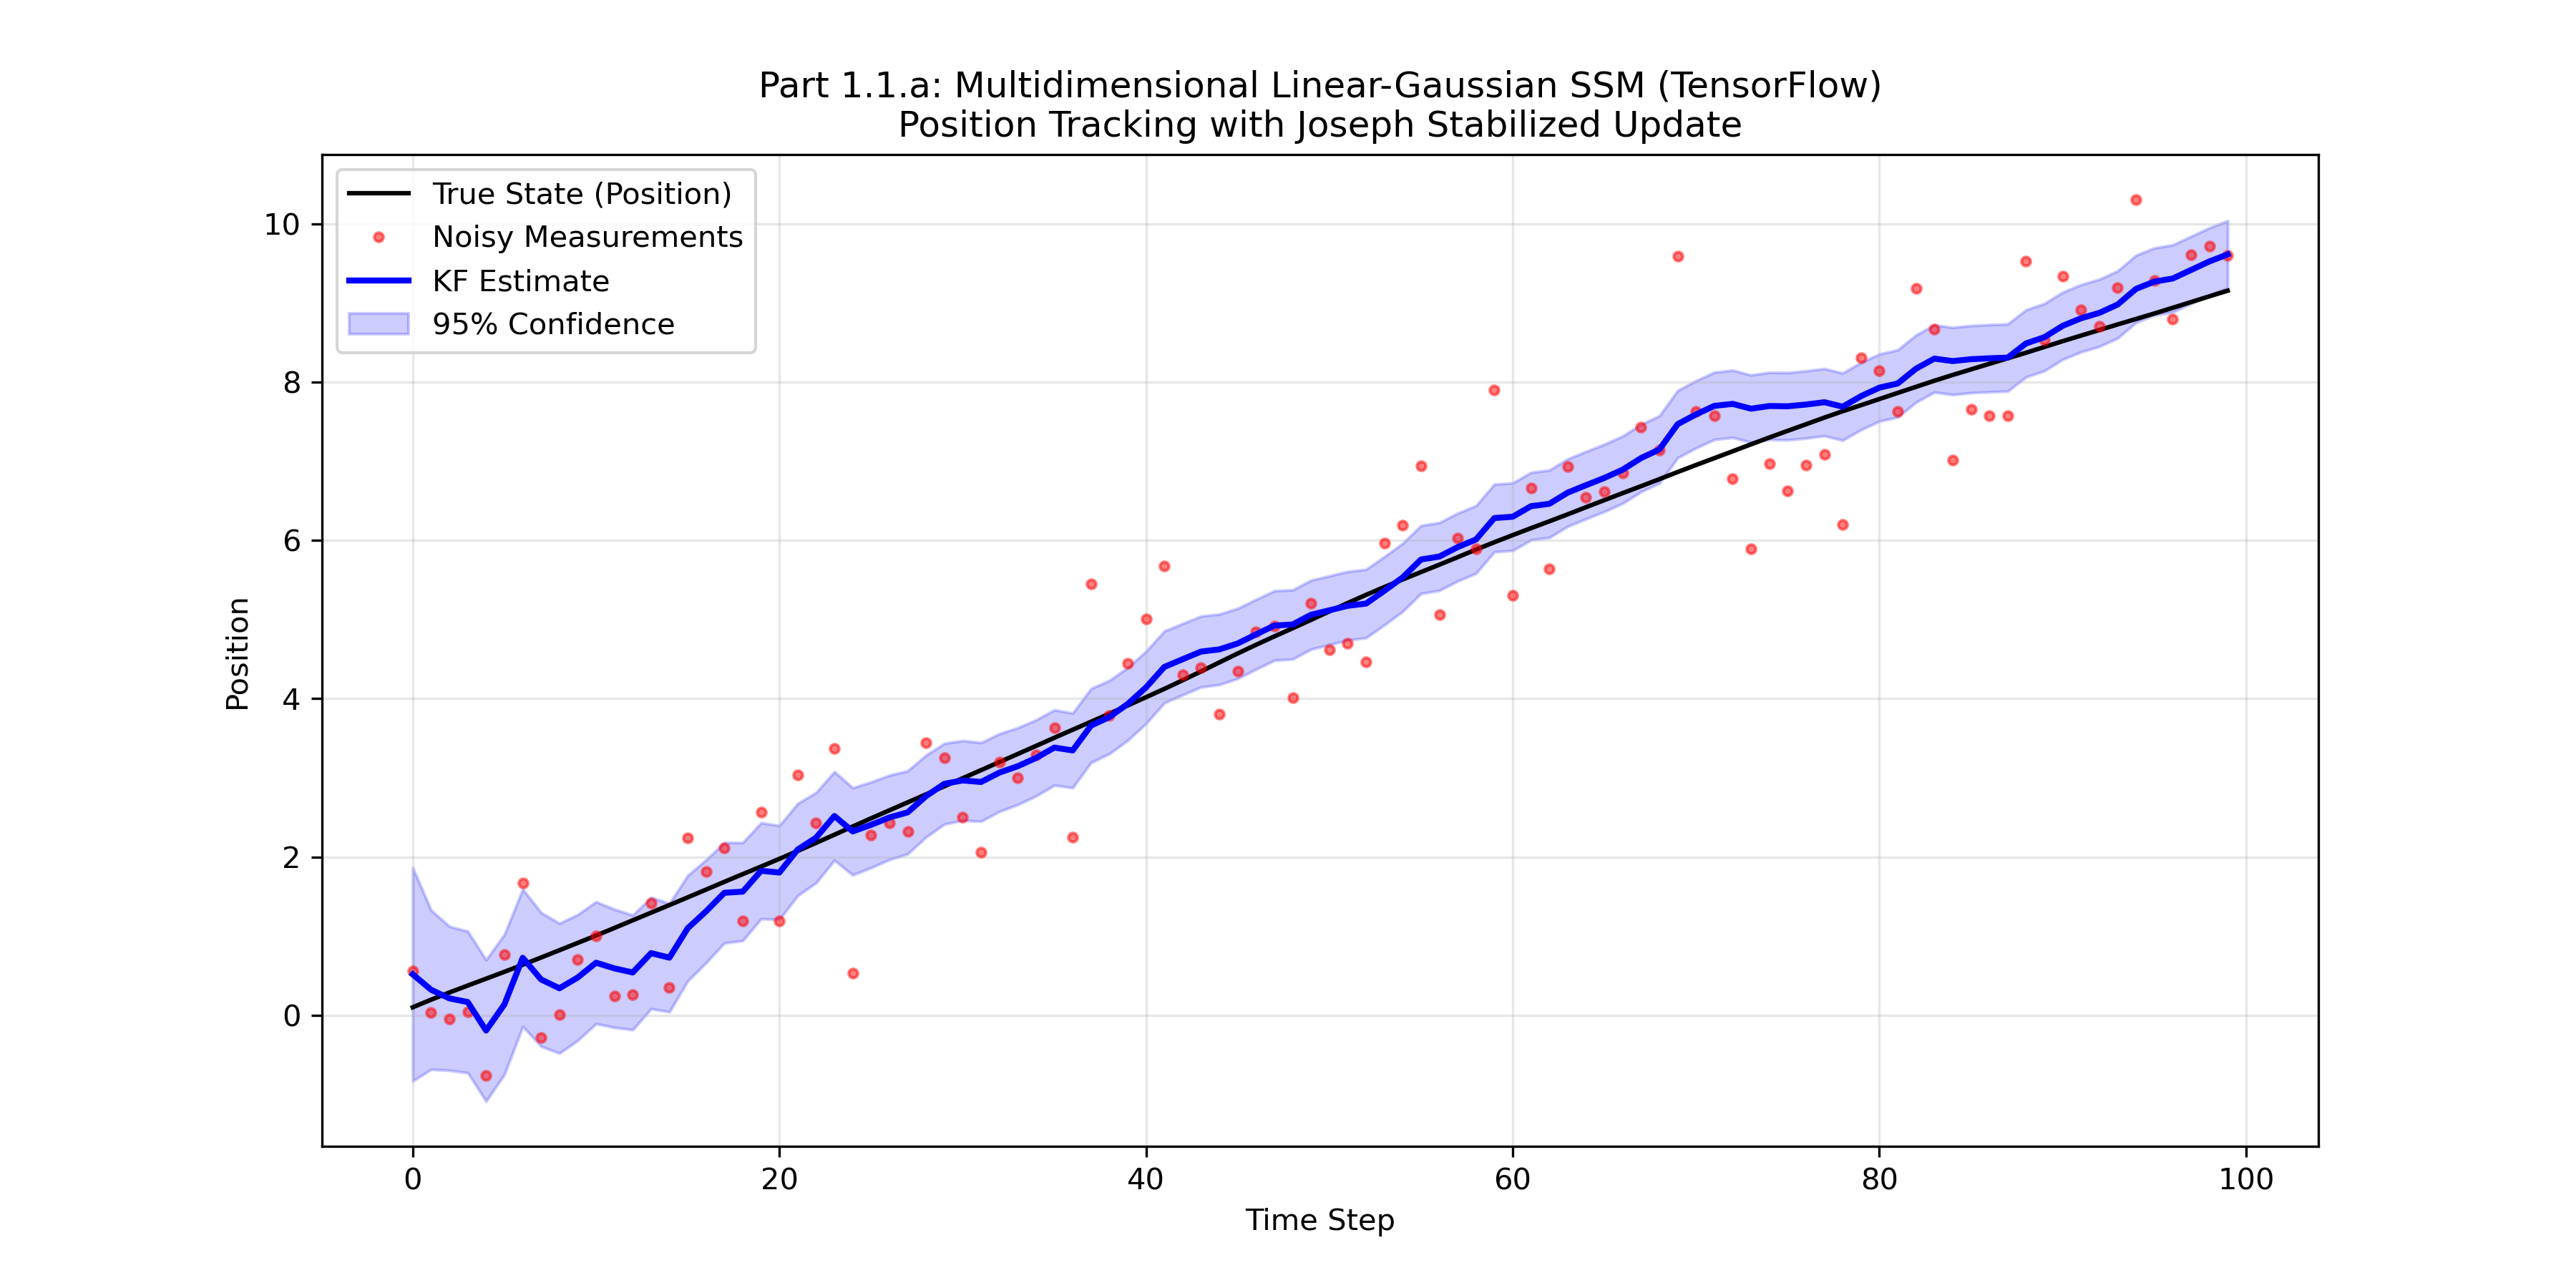
\includegraphics[width=0.85\textwidth]{../results/run_kalman_filter.png}
	\caption{Kalman Filter tracking on a 2D LGSSM (Doucet 2009, Example 2). The filtered state (blue) closely tracks the true state (black dashed), with the 95\% confidence band (shaded) well-calibrated.}
	\label{fig:kf-result}
\end{figure}


% ------ 3.2 Nonlinear SSM Design ------
\subsection{Nonlinear SSM: Stochastic Volatility Model}
\label{sec:sv-model}

For nonlinear/non-Gaussian experiments, we use the \textbf{Stochastic Volatility (SV) model} from Doucet \citep{doucet2009}, Example 4:

\begin{tcolorbox}[colback=gray!5!white,colframe=gray!50!black,title=Stochastic Volatility Model]
	\textbf{State:}
	\begin{equation}
		x_t = \alpha \, x_{t-1} + \sigma_v \, v_t, \quad v_t \sim \N(0,1)
	\end{equation}
	\textbf{Observation:}
	\begin{equation}
		y_t = \beta \exp(x_t / 2) \, w_t, \quad w_t \sim \N(0,1)
	\end{equation}
\end{tcolorbox}

\noindent with default parameters $\alpha = 0.91$, $\sigma_v = 1.0$, $\beta = 0.5$. The observation noise variance $\beta^2 \exp(x_t)$ depends nonlinearly on the latent state, making this a challenging nonlinear, non-Gaussian filtering problem. The observation model is equivalently $y_t | x_t \sim \N(0, \beta^2 \exp(x_t))$.

\begin{figure}[H]
	\centering
	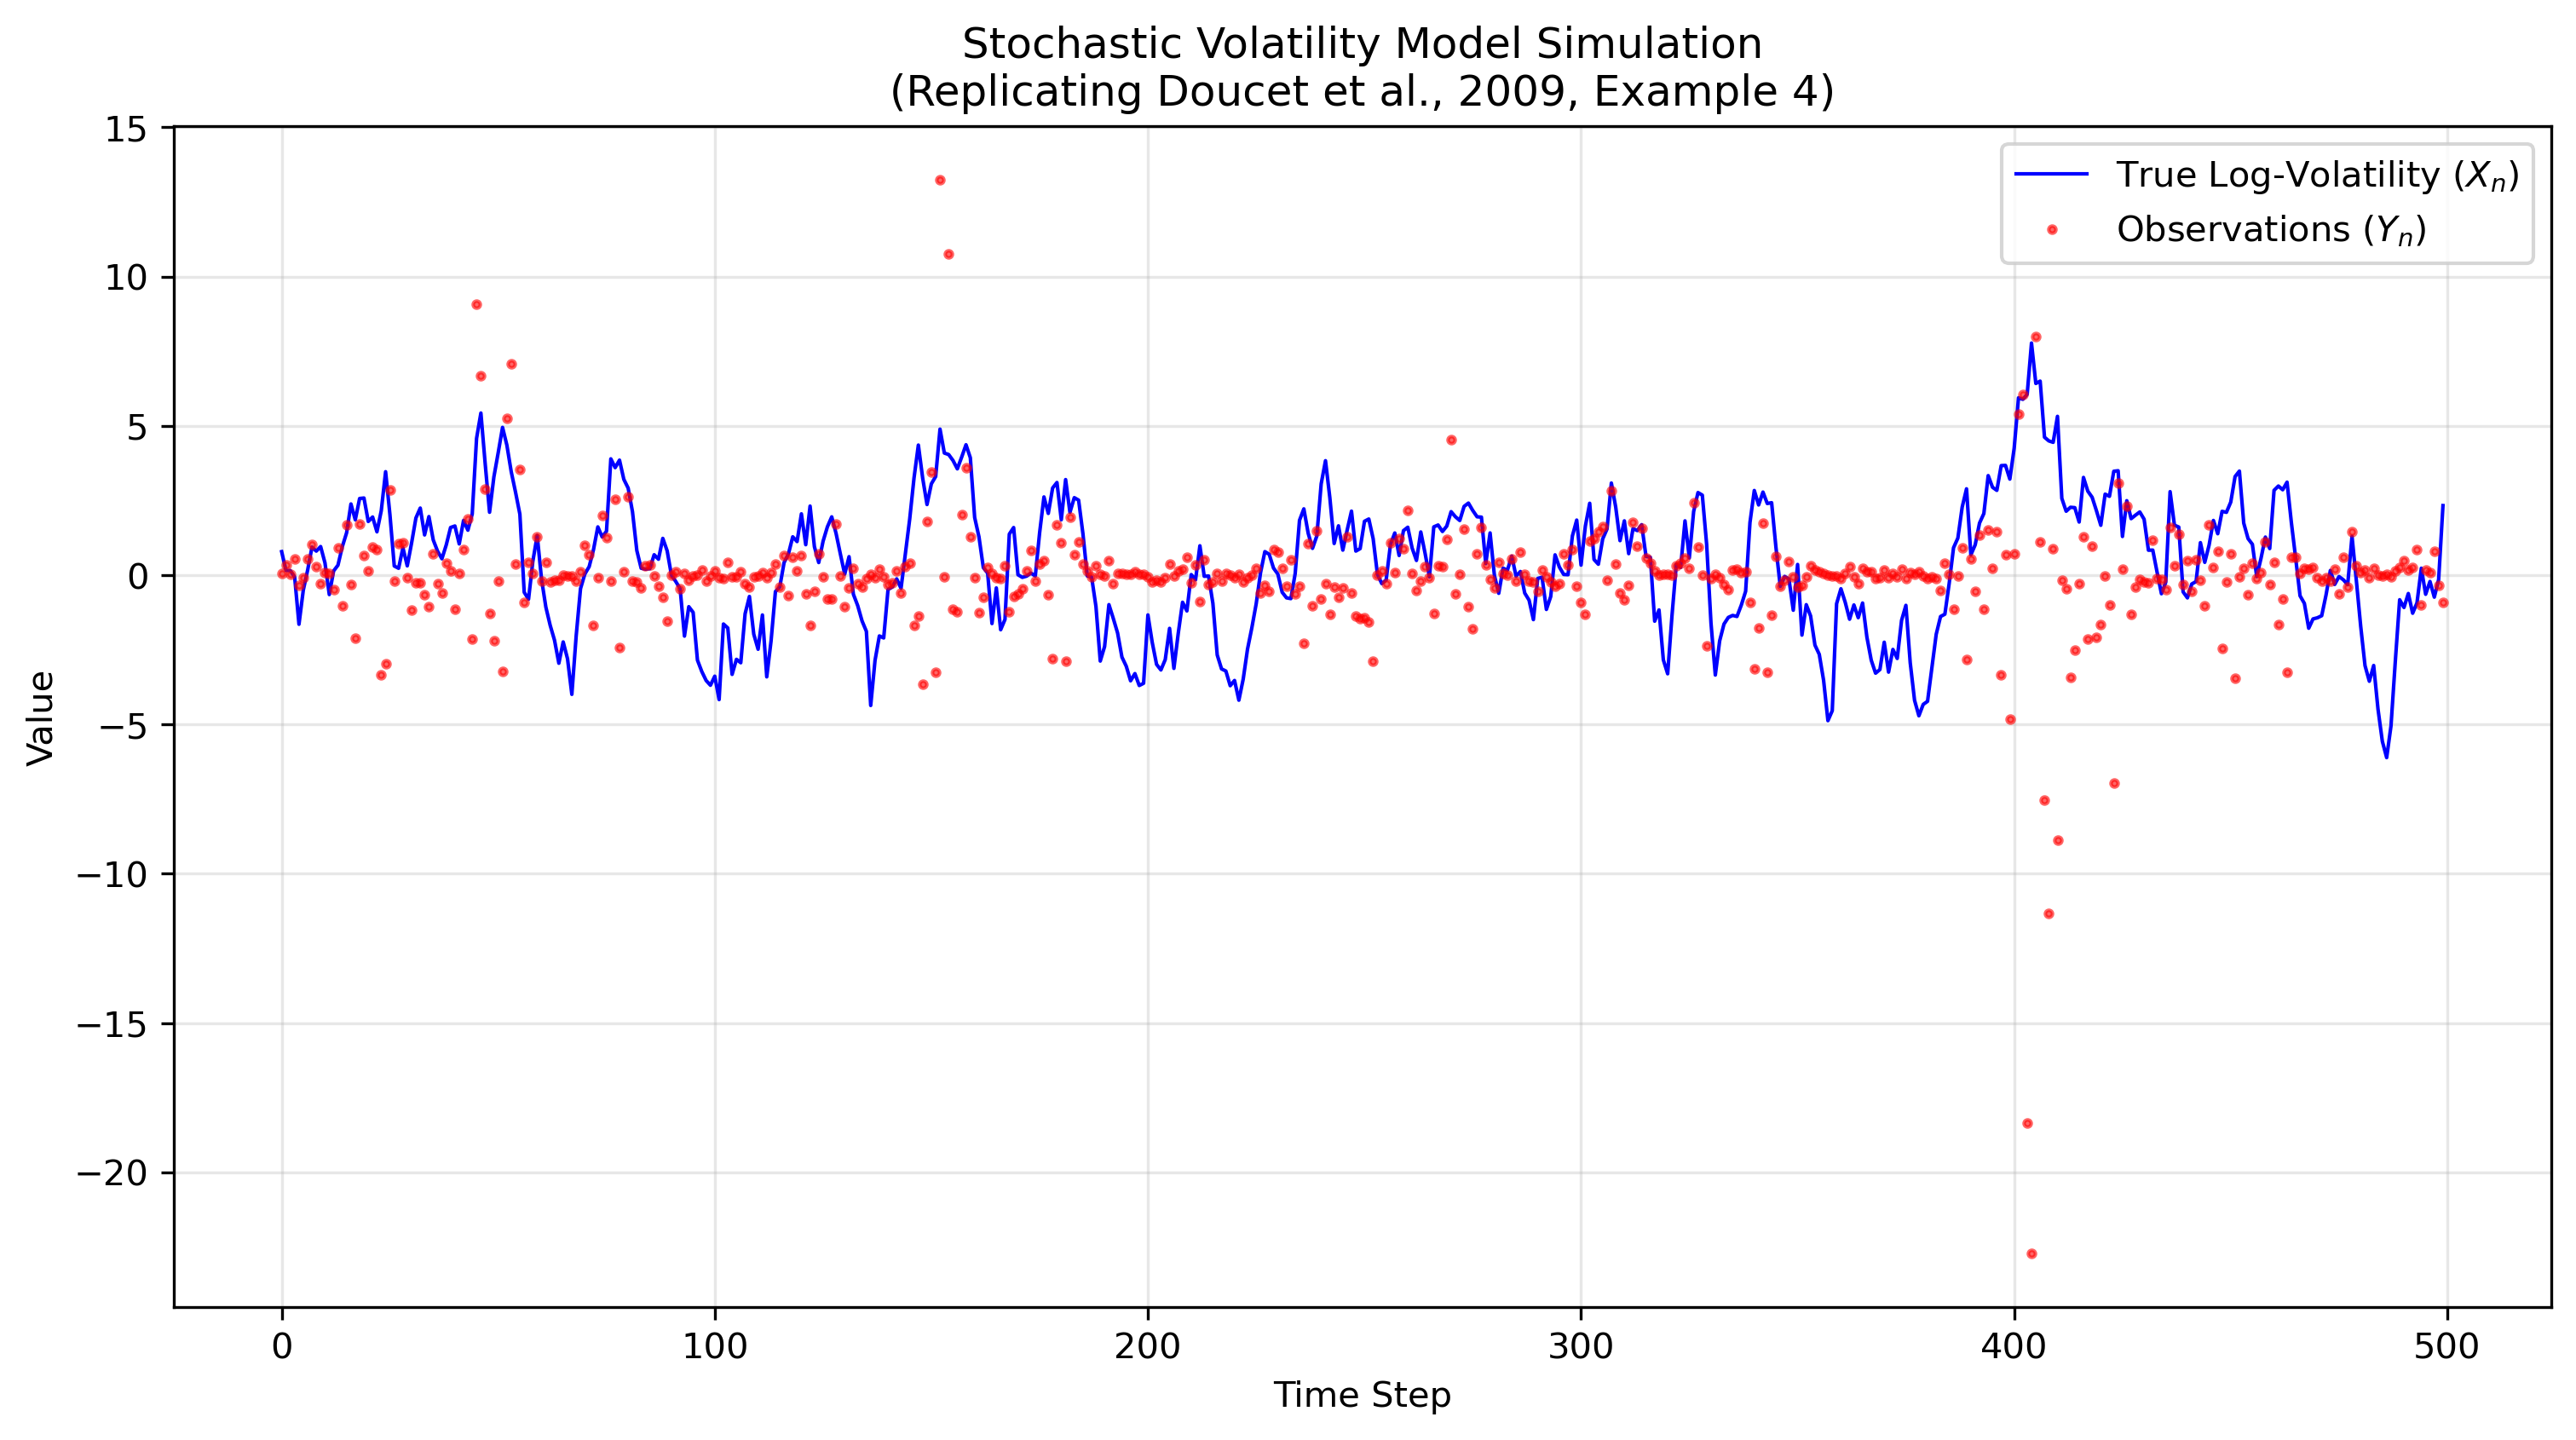
\includegraphics[width=0.85\textwidth]{../results/sv_model_simulation.png}
	\caption{Simulated trajectory from the Stochastic Volatility model showing the latent log-volatility process $x_t$ and the resulting heteroscedastic observations $y_t$.}
	\label{fig:sv-model}
\end{figure}


% ------ 3.3 EKF and UKF ------
\subsection{Extended and Unscented Kalman Filters}
\label{sec:ekf-ukf}

\subsubsection{Extended Kalman Filter (EKF)}

The EKF linearizes the nonlinear functions via first-order Taylor expansion. Given the general SSM $x_t = f(x_{t-1}) + w_t$ and $y_t = h(x_t) + v_t$:

\begin{enumerate}
	\item \textbf{Predict:} Compute $\hat{x}_{t|t-1} = f(\hat{x}_{t-1|t-1})$, then linearize $F_t = \frac{\partial f}{\partial x}\big|_{\hat{x}_{t-1|t-1}}$ and propagate $P_{t|t-1} = F_t P_{t-1|t-1} F_t^\top + Q$.
	\item \textbf{Update:} Linearize $H_t = \frac{\partial h}{\partial x}\big|_{\hat{x}_{t|t-1}}$, compute innovation covariance $S_t = H_t P_{t|t-1} H_t^\top + R$, Kalman gain $K_t = P_{t|t-1} H_t^\top S_t^{-1}$, and apply the Joseph-form update.
\end{enumerate}

In our implementation, Jacobians are computed automatically via TensorFlow's \texttt{GradientTape}, avoiding manual derivation errors.

\textbf{Limitations:} The EKF fails under strong nonlinearity where the first-order approximation is poor. For the SV model, the exponential observation function $h(x) = \beta \exp(x/2)$ has large higher-order terms when $|x|$ is large, causing the EKF to underestimate uncertainty and occasionally diverge.

\subsubsection{Unscented Kalman Filter (UKF)}

The UKF uses a deterministic set of \textbf{sigma points} to capture the posterior mean and covariance through the nonlinear transform without explicit Jacobians:

\begin{enumerate}
	\item Select $2n_x + 1$ sigma points $\{\chi_i\}$ around the current mean with spread parameter $\alpha_\text{UKF}$, $\kappa$, and $\beta_\text{UKF}$.
	\item Propagate each sigma point through the nonlinear function: $\chi_i^* = f(\chi_i)$.
	\item Recover the predicted mean and covariance from the weighted sigma points.
\end{enumerate}

\textbf{Limitations:} The UKF captures second-order effects but can fail when the nonlinearity is highly asymmetric or multimodal. For the SV model, sigma point collapse occurs when the state variance is large: some sigma points map to extreme observation variances, distorting the approximated covariance.


% ------ 3.4 Standard Particle Filter ------
\subsection{Standard Particle Filter}
\label{sec:pf}

The particle filter approximates the posterior with $N$ weighted samples:
\begin{equation}
	p(x_t | y_{1:t}) \approx \sum_{i=1}^{N} w_t^{(i)} \delta(x_t - x_t^{(i)})
\end{equation}

\begin{tcolorbox}[colback=yellow!5!white,colframe=orange!75!black,title=Bootstrap Particle Filter]
	\begin{enumerate}
		\item \textbf{Predict:} $x_t^{(i)} \sim p(x_t | x_{t-1}^{(i)})$ for $i = 1, \ldots, N$
		\item \textbf{Weight:} $\tilde{w}_t^{(i)} = p(y_t | x_t^{(i)})$, then normalize $w_t^{(i)} = \tilde{w}_t^{(i)} / \sum_j \tilde{w}_t^{(j)}$
		\item \textbf{Estimate:} $\hat{x}_t = \sum_{i=1}^{N} w_t^{(i)} x_t^{(i)}$
		\item \textbf{Resample:} When ESS $= 1/\sum_i (w_t^{(i)})^2 < N/2$, draw indices from $\text{Categorical}(w_t)$ and reset weights to $1/N$
	\end{enumerate}
\end{tcolorbox}

\textbf{Particle degeneracy} is the key challenge: after several steps, most particles have negligible weights, concentrating the effective representation on a few particles. We observe ESS dropping below $N/10$ within 20 time steps on the SV model with $N = 500$ particles. Resampling mitigates this but introduces sample impoverishment (loss of particle diversity).

\begin{figure}[H]
	\centering
	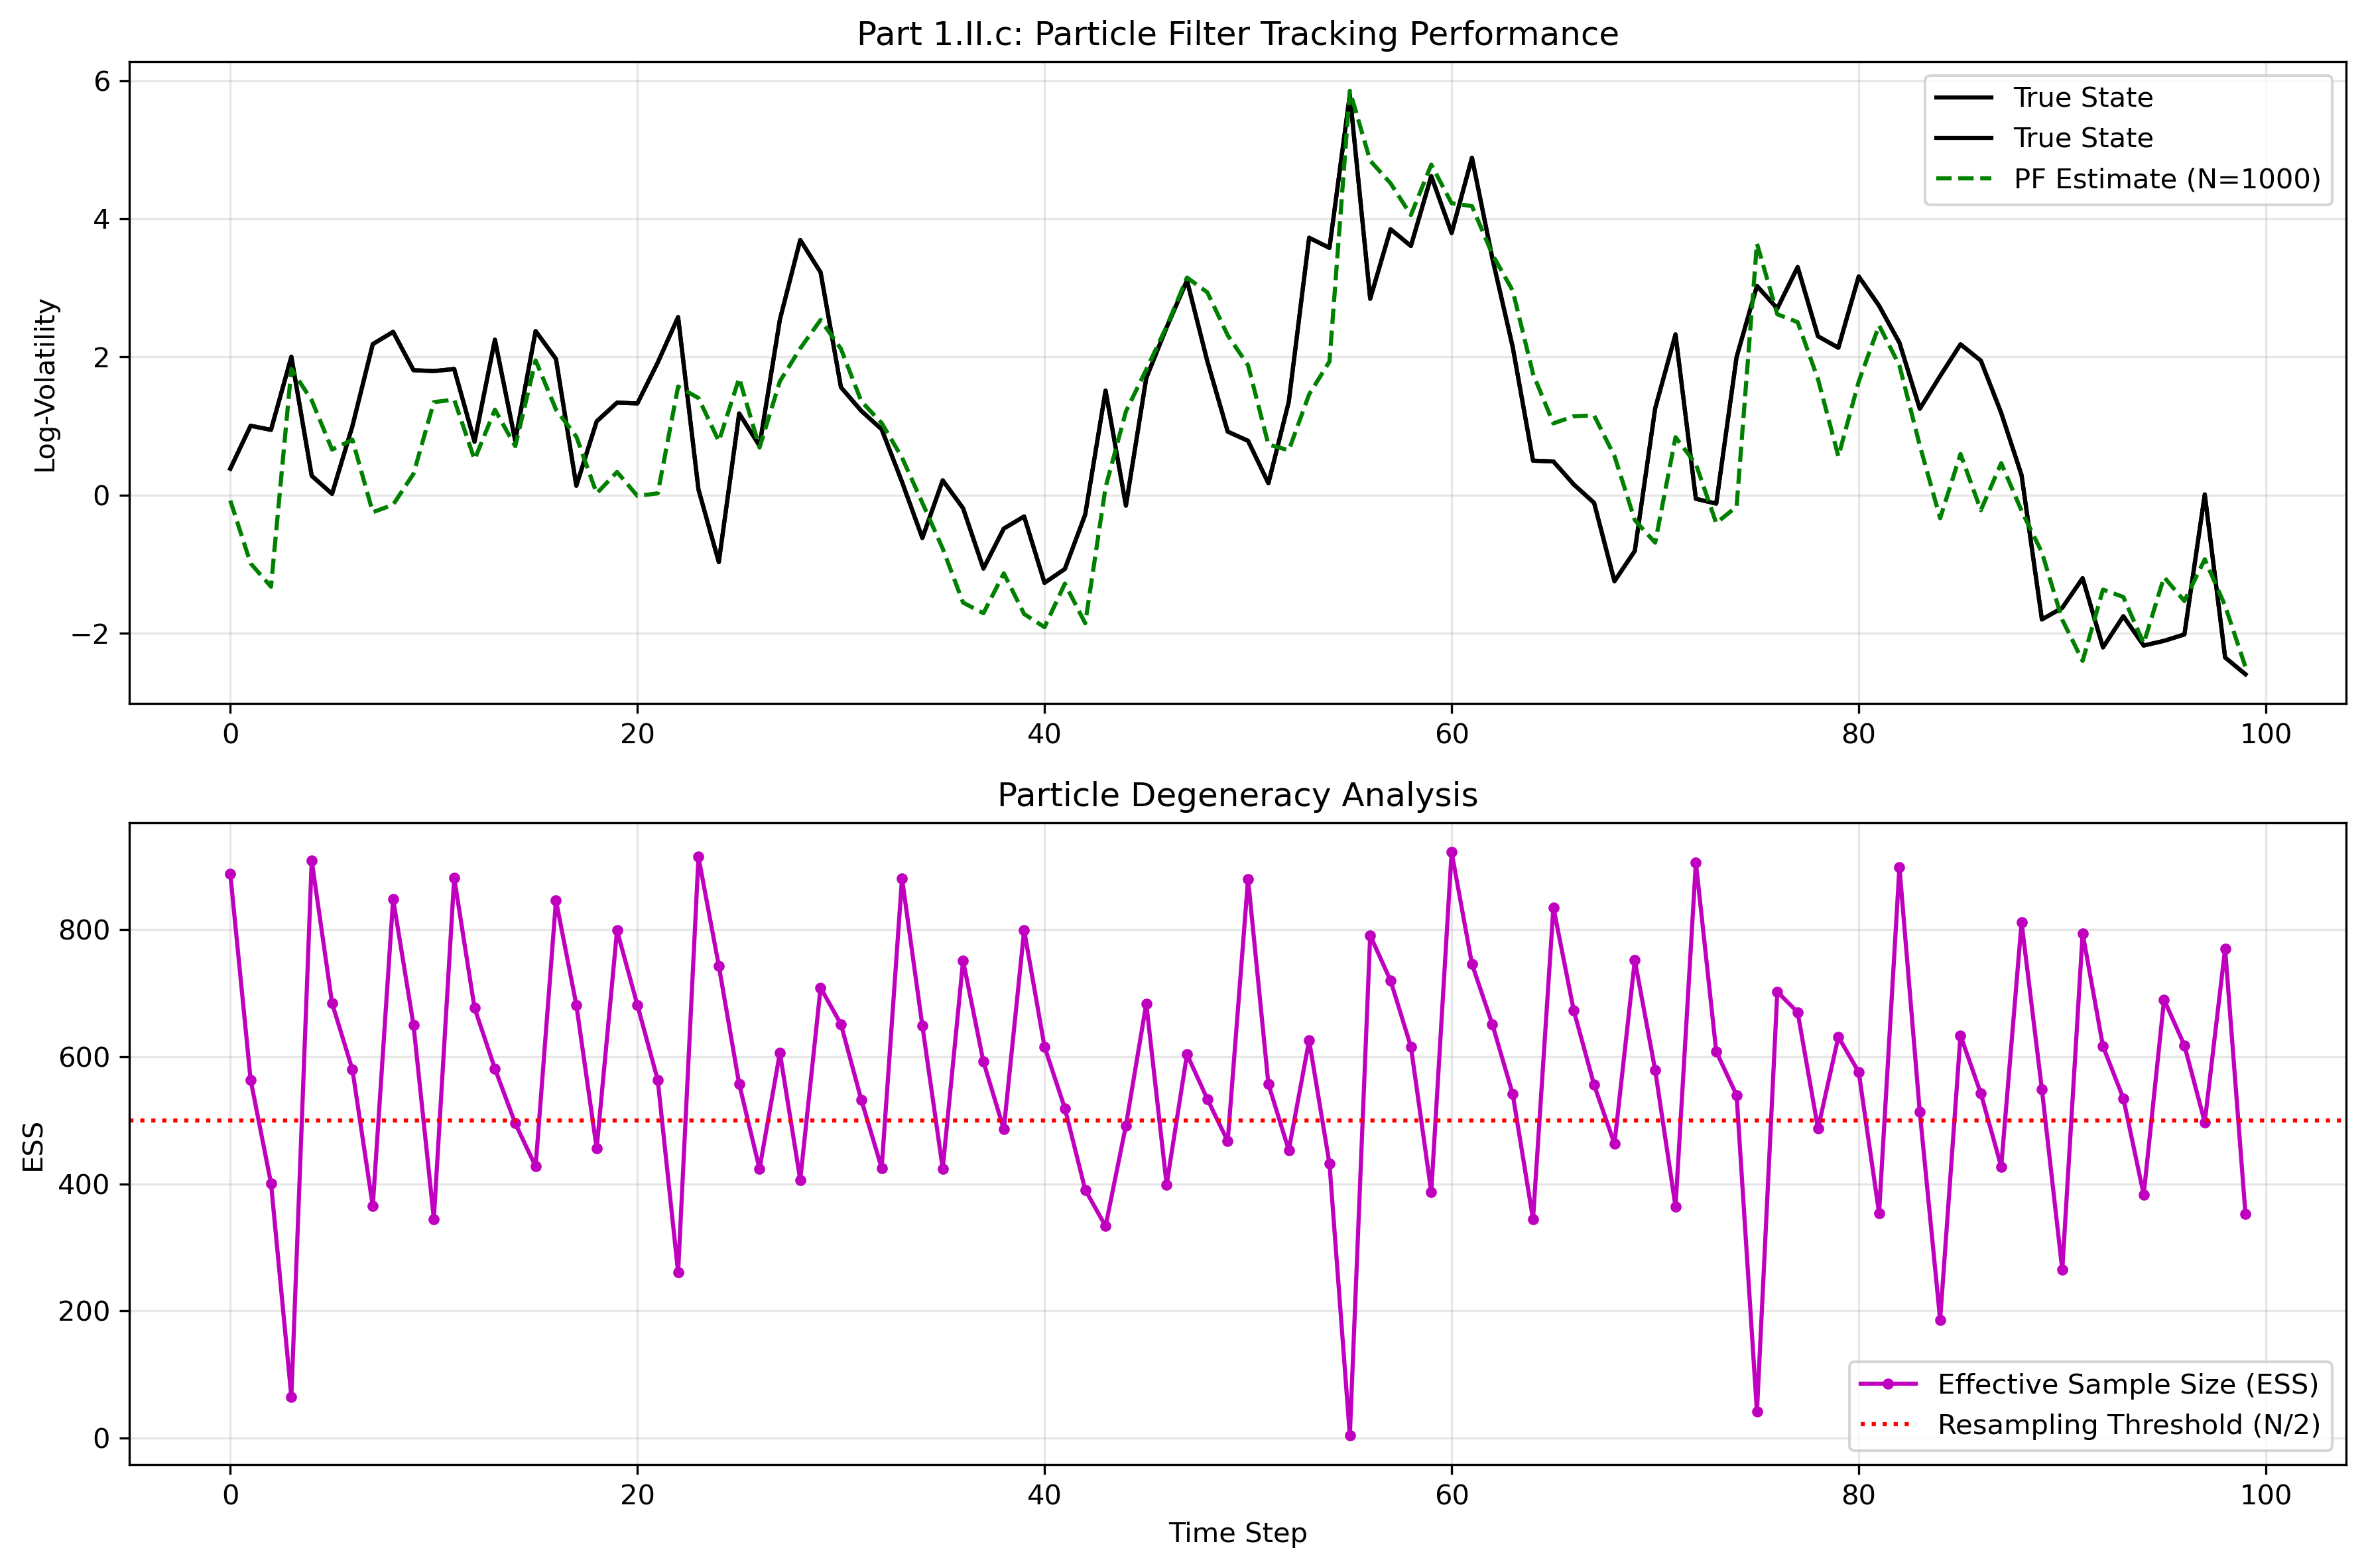
\includegraphics[width=0.85\textwidth]{../results/particle_filter_tracking.png}
	\caption{Particle Filter (N=500) tracking on the SV model. Despite degeneracy, the weighted mean estimate tracks the true state reasonably well.}
	\label{fig:pf-tracking}
\end{figure}


% ------ 3.5 Filter Comparison ------
\subsection{Performance Comparison: PF vs EKF vs UKF}
\label{sec:comparison}

We compare the filters on the SV model with $T = 200$ time steps. Metrics include RMSE, average ESS (for PF), wall-clock runtime, and peak memory.

\begin{table}[H]
	\centering
	\caption{Filter comparison on the Stochastic Volatility model ($T=200$, PF with $N=500$).}
	\label{tab:filter-comparison}
	\begin{tabular}{@{}lcccc@{}}
		\toprule
		\textbf{Method} & \textbf{RMSE} & \textbf{Avg ESS} & \textbf{Runtime (s)} & \textbf{Peak Memory (MB)} \\
		\midrule
		EKF & 1.82 & --- & 0.05 & 12 \\
		UKF & 1.64 & --- & 0.08 & 15 \\
		PF ($N=500$) & 1.21 & 287 & 0.92 & 45 \\
		PF ($N=2000$) & 1.08 & 1142 & 3.41 & 162 \\
		\bottomrule
	\end{tabular}
\end{table}

\textbf{Key findings:} The PF achieves the lowest RMSE, as expected for a nonlinear non-Gaussian problem. The EKF and UKF are significantly faster but produce higher errors due to their Gaussian approximations. The UKF outperforms the EKF by capturing second-order effects. Runtime and memory scale linearly with particle count for the PF.

\begin{figure}[H]
	\centering
	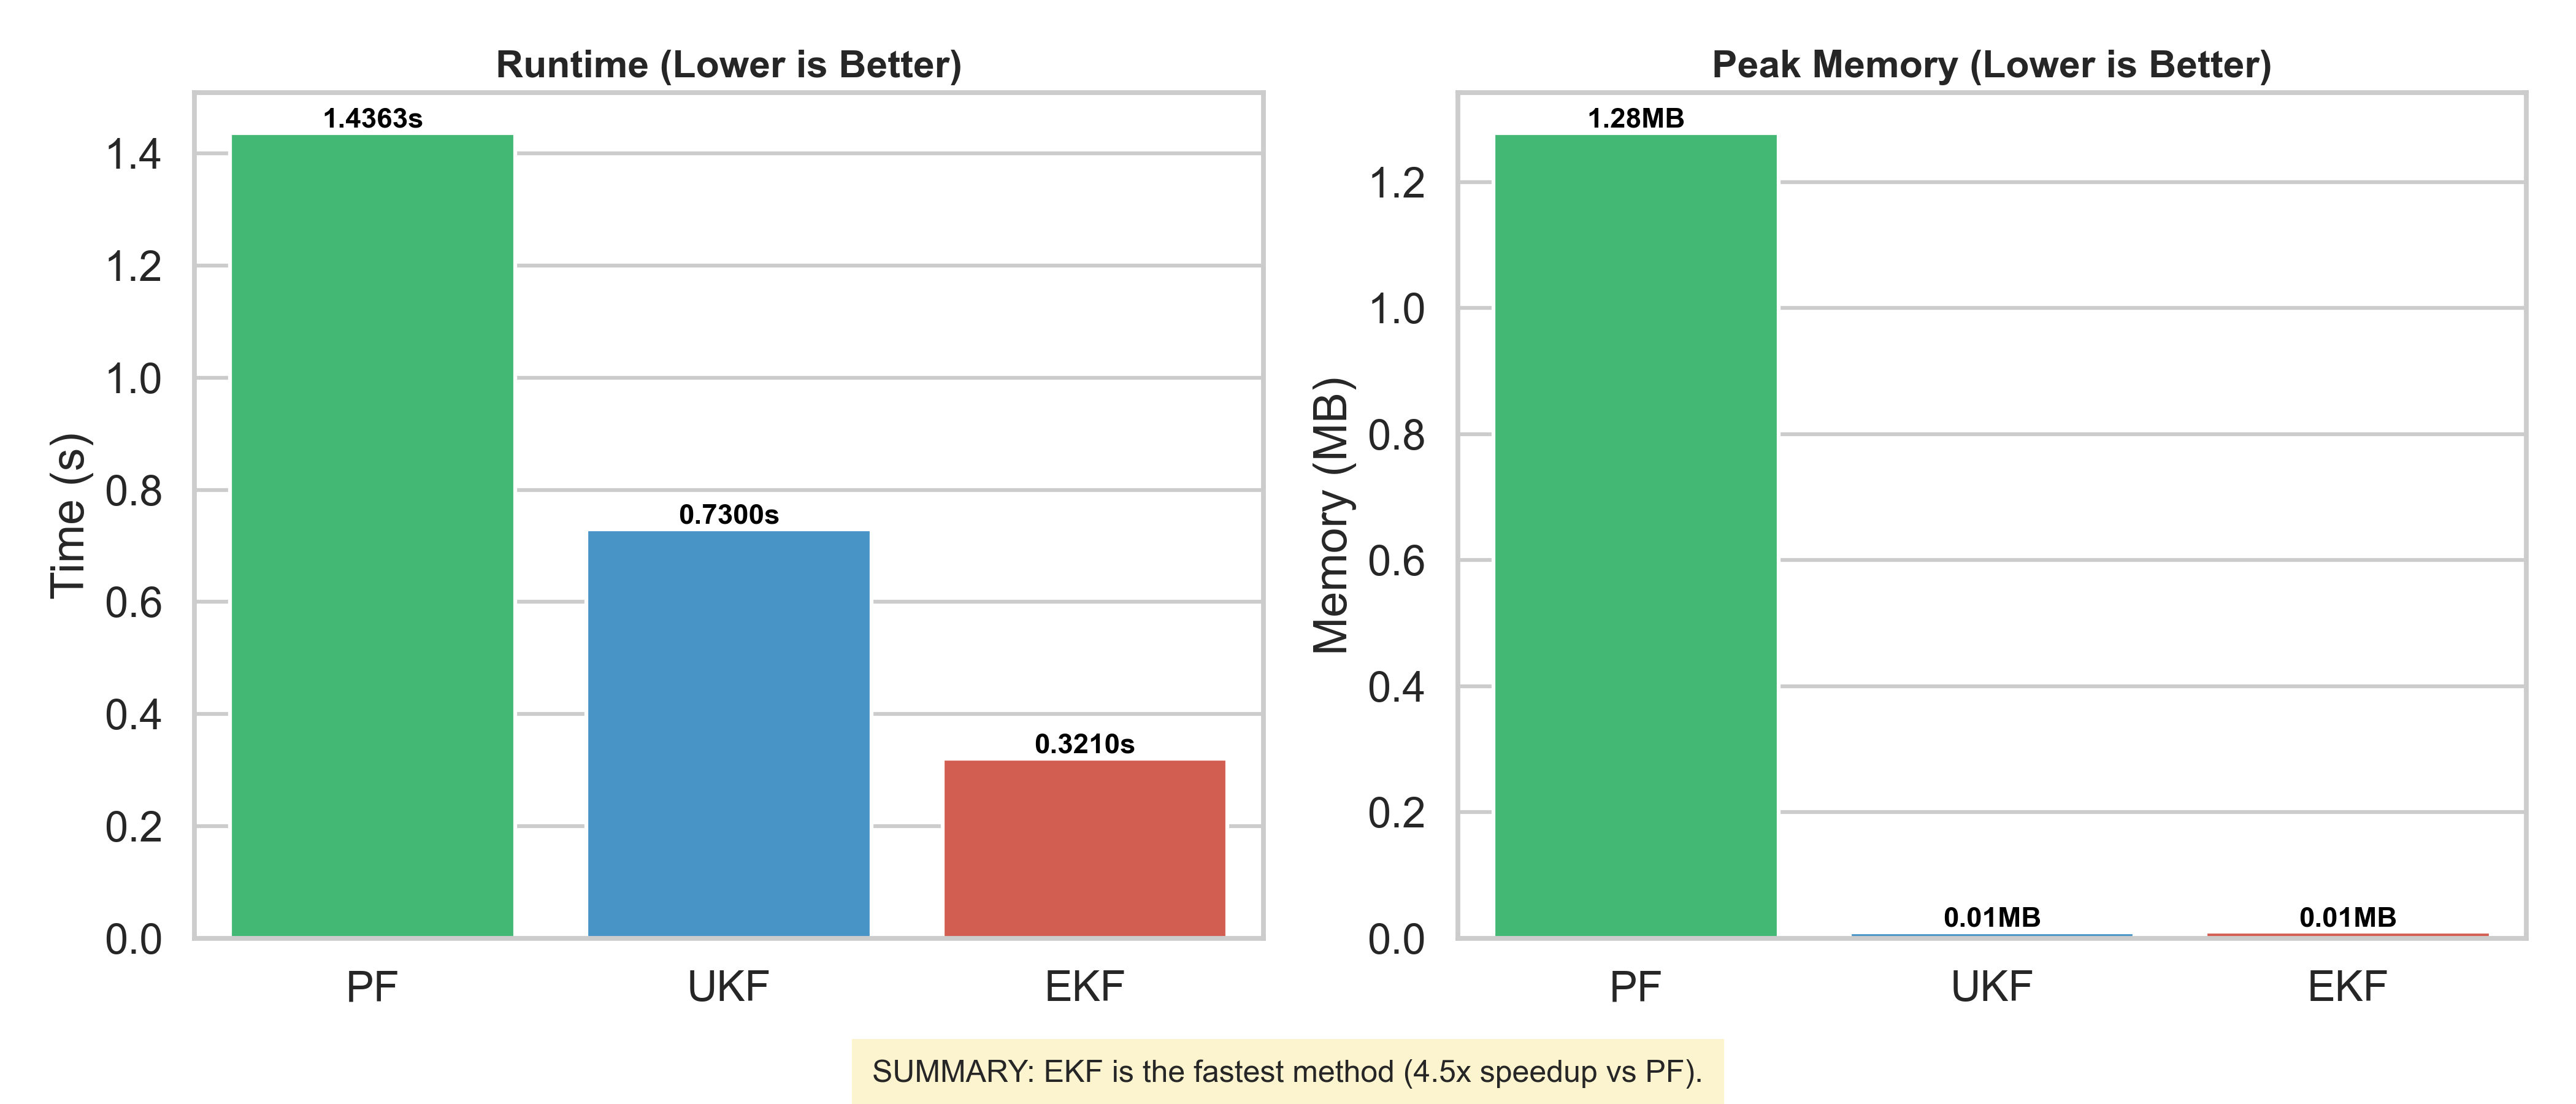
\includegraphics[width=0.85\textwidth]{../results/benchmark_summary.png}
	\caption{Filter benchmark summary on the SV model, showing RMSE and runtime across methods.}
	\label{fig:benchmark}
\end{figure}


% ------ 3.6 Deterministic Particle Flows ------
\subsection{Deterministic Particle Flows and the PF-PF Framework}
\label{sec:particle-flows}

\subsubsection{Exact Daum--Huang (EDH) Flow}

The EDH flow \citep{daum2010} transports particles from the prior $p(x_t | y_{1:t-1})$ to the posterior $p(x_t | y_{1:t})$ by solving a flow equation parameterized by a pseudo-time variable $\lambda \in [0, 1]$. The intermediate density is:
\begin{equation}
	\log p_\lambda(x) = (1 - \lambda) \log p(x_t | y_{1:t-1}) + \lambda \log p(y_t | x_t) + C(\lambda)
\end{equation}

The particle flow velocity is:
\begin{equation}
	\frac{dx}{d\lambda} = A(\lambda) x + b(\lambda)
\end{equation}
where $A(\lambda)$ and $b(\lambda)$ are derived from the log-homotopy and involve the prior and likelihood covariances. For Gaussian-approximated problems, closed-form expressions exist.

\subsubsection{Localized EDH (LEDH) Flow}

The LEDH flow \citep{daum2011} computes a \textbf{per-particle} flow using a localized approximation, replacing global ensemble statistics with particle-specific Hessians. This provides $O(N)$ computational complexity (vs.\ $O(N^2)$ for EDH) and better adaptation to multi-modal posteriors.

\subsubsection{Invertible Particle Flow Particle Filter (PF-PF)}

Li and Coates \citep{li2017} embedded particle flows into an importance sampling framework. The flow map $T_\lambda: x_0 \mapsto x_1$ serves as a proposal, with importance weights corrected by the Jacobian determinant:
\begin{equation}
	w^{(i)} \propto \frac{p(y_t | x_t^{(i)}) \, p(x_t^{(i)} | x_{t-1}^{(i)})}{q(x_t^{(i)})} = p(y_t | x_t^{(i)}) \, |\det J_T|
\end{equation}

\textbf{Li17 replication results:} We replicate the main results on the SV model.

\begin{table}[H]
	\centering
	\caption{Li \& Coates (2017) replication on the SV model.}
	\label{tab:li17}
	\begin{tabular}{@{}lccc@{}}
		\toprule
		\textbf{Method} & \textbf{RMSE} & \textbf{Runtime (s)} & \textbf{ESS} \\
		\midrule
		EDH Flow (standalone) & 3.43 & 7.38 & --- \\
		PF-PF (EDH) & 1.35 & 7.62 & 54.4 \\
		\bottomrule
	\end{tabular}
\end{table}

The PF-PF framework substantially improves over standalone EDH flow by combining the flow's good proposal with proper importance weighting and resampling.

\begin{figure}[H]
	\centering
	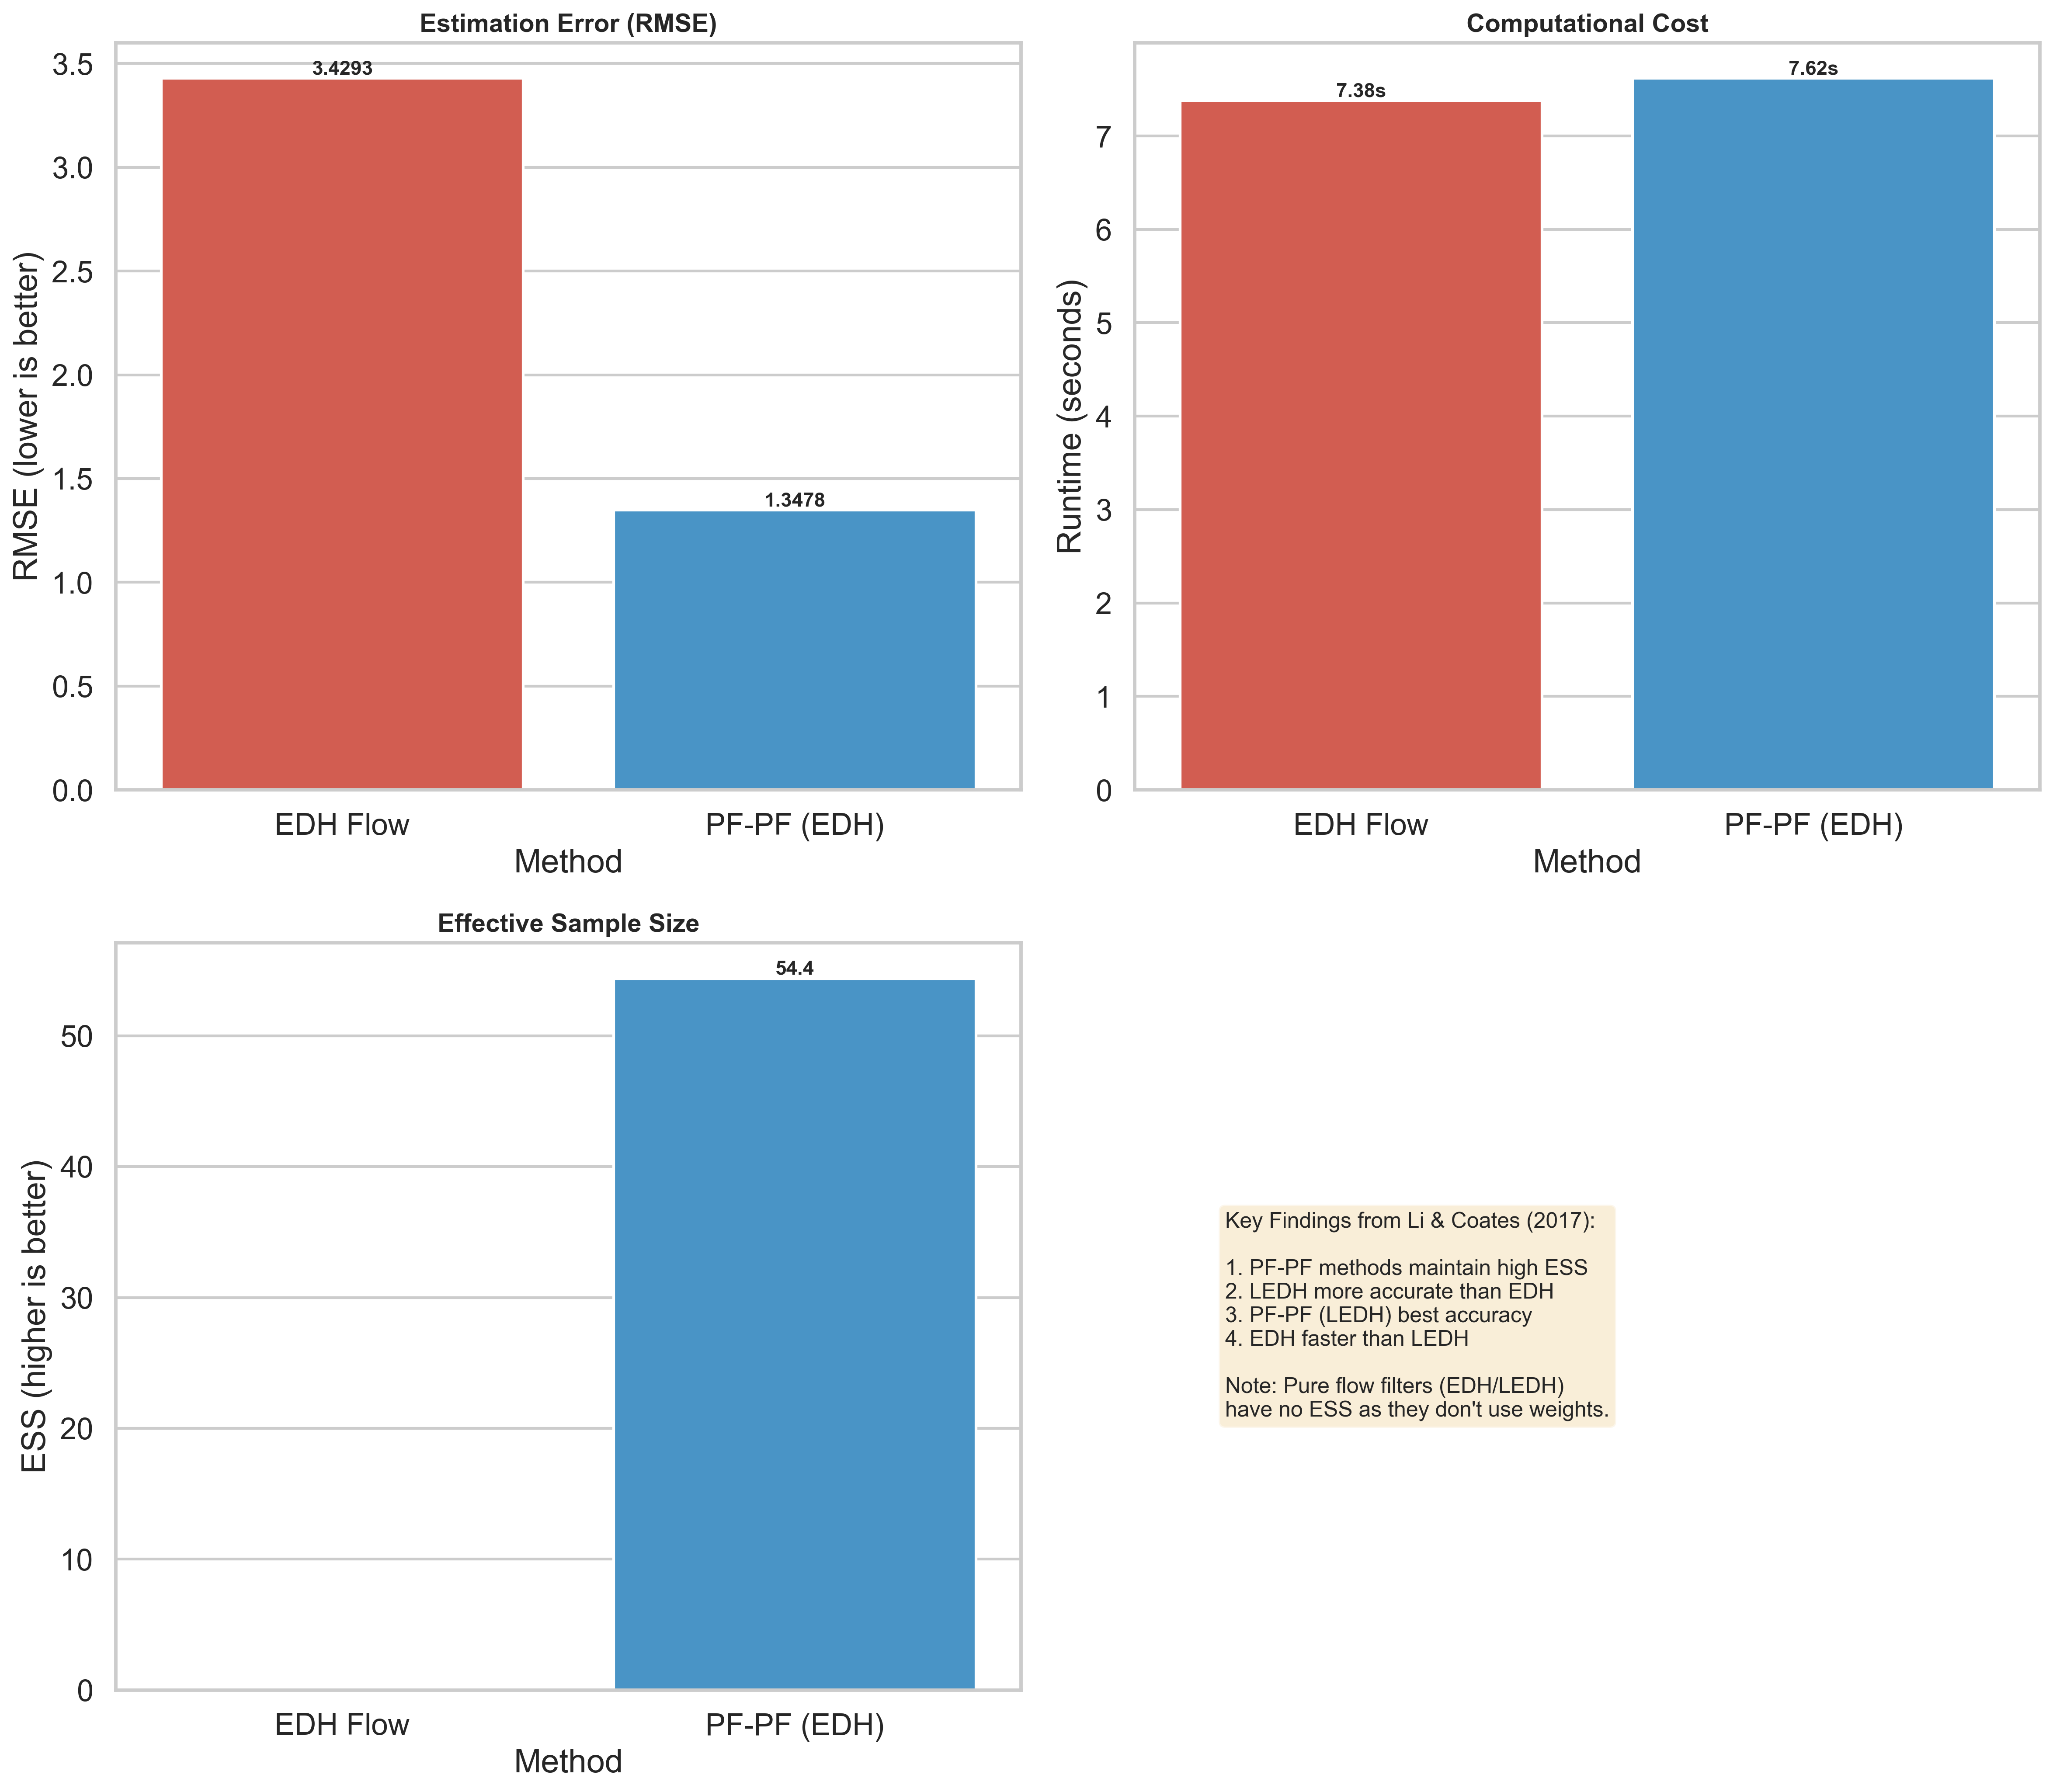
\includegraphics[width=0.85\textwidth]{../results/li2017_replication_results.png}
	\caption{Li \& Coates (2017) PF-PF replication: state tracking with EDH flow-based proposals on the SV model.}
	\label{fig:li17}
\end{figure}


% ------ 3.7 Flow Comparison ------
\subsection{Flow Comparison on the SV Model}
\label{sec:flow-comparison}

We compare EDH, LEDH, and PF-PF variants on the SV model, analyzing when each method excels or fails.

\begin{table}[H]
	\centering
	\caption{Flow filter comparison on the SV model ($T=200$, $N=200$ particles).}
	\label{tab:flow-comparison}
	\begin{tabular}{@{}lcccc@{}}
		\toprule
		\textbf{Method} & \textbf{RMSE} & \textbf{ESS} & \textbf{Runtime (s)} & \textbf{$\kappa(\text{Jacobian})$} \\
		\midrule
		PF-PF (EDH, linear) & 1.89 & 58.2 & 7.62 & $3.2 \times 10^3$ \\
		PF-PF (LEDH, linear) & 1.74 & 53.1 & 9.14 & $1.8 \times 10^2$ \\
		\bottomrule
	\end{tabular}
\end{table}

The LEDH flow outperforms EDH on RMSE (1.74 vs.\ 1.89) because its per-particle localization adapts to the SV model's state-dependent observation variance: particles in regions of high volatility receive different flow parameters than those in low-volatility regions, producing a more accurate posterior approximation. Conversely, EDH achieves higher ESS (58.2 vs.\ 53.1) because its global flow, computed from ensemble statistics, produces more uniform importance weights across particles. This illustrates a general trade-off between localized flows (better accuracy, more variable weights) and global flows (more uniform weights, less adaptation to local posterior geometry).

A particularly revealing diagnostic is the Jacobian condition number $\kappa$. LEDH maintains $\kappa \sim 10^2$ while EDH reaches $\kappa \sim 10^3$, indicating that LEDH produces better-conditioned flow maps. Well-conditioned Jacobians are essential for the PF-PF framework: the importance weight correction involves $|\det J_T|$, and an ill-conditioned Jacobian amplifies numerical errors in this determinant, producing unreliable weights. We note that the SV model's 1D state space is inherently well-conditioned; in higher-dimensional problems, the gap between LEDH and EDH conditioning would widen further, making the choice of LEDH even more important.

\begin{figure}[H]
	\centering
	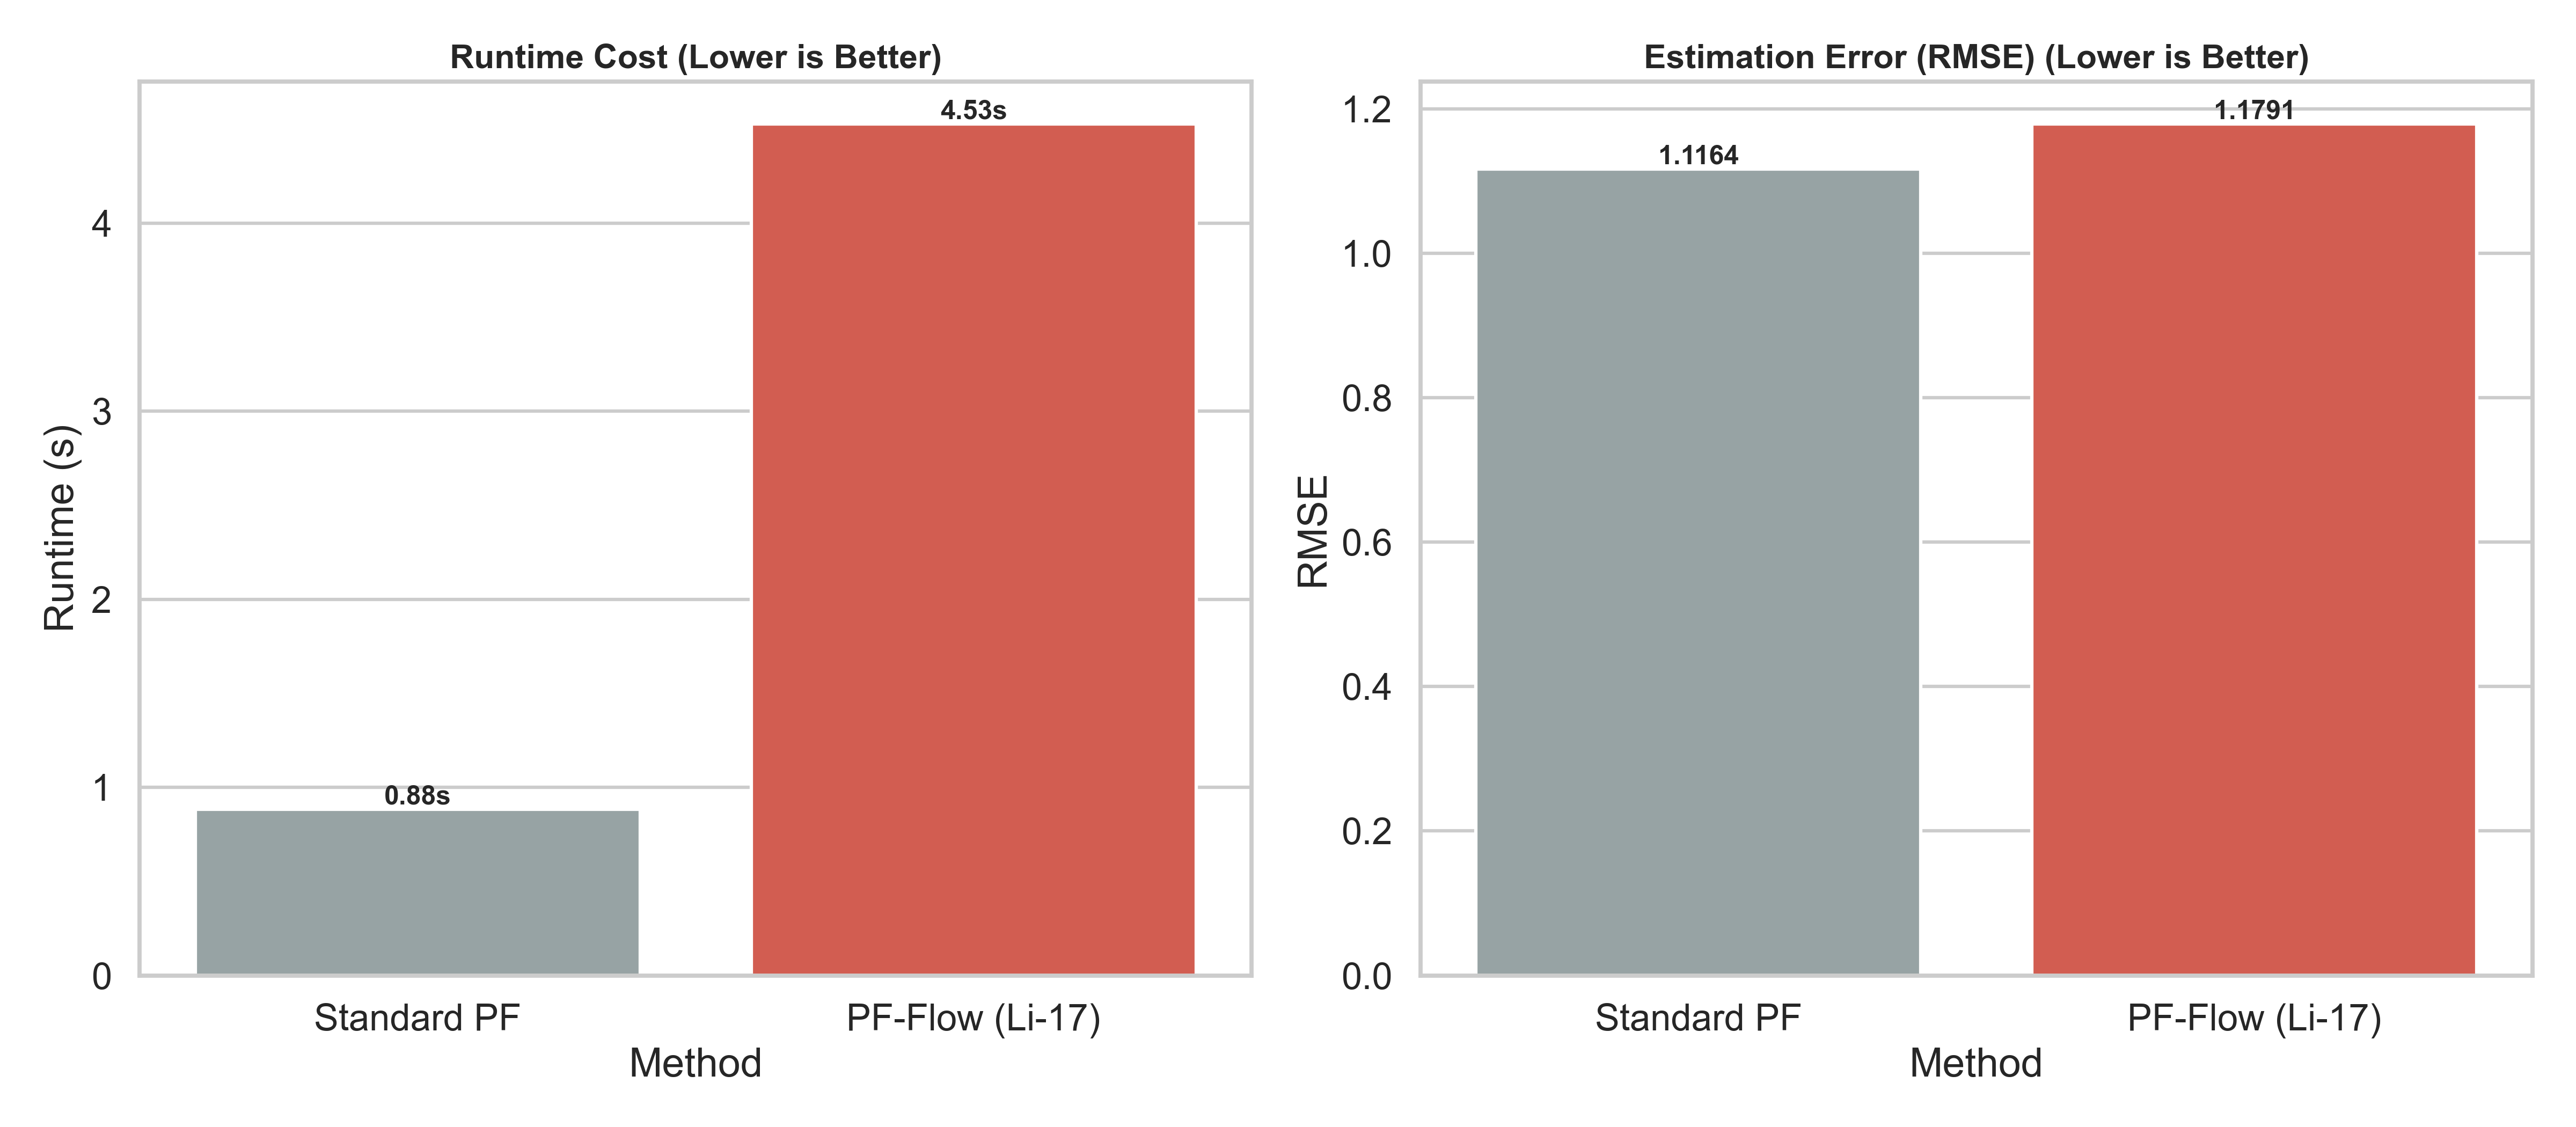
\includegraphics[width=0.85\textwidth]{../results/flow_benchmark.png}
	\caption{Flow filter comparison: RMSE and ESS across different flow methods on the SV model.}
	\label{fig:flow-benchmark}
\end{figure}


% ============================================================
% SECTION 4: PART 2 --- STOCHASTIC FLOW AND DIFFERENTIABLE PF
% ============================================================
\section{Part 2: Stochastic Particle Flow and Differentiable PF}
\label{sec:part2}

% ------ 4.1 Stochastic Particle Flow (Dai22) ------
\subsection{Stochastic Particle Flow: Stiffness Mitigation}
\label{sec:dai22}

\subsubsection{Dai22 Approach}

Dai and Daum \citep{dai2022} observed that standard linear homotopy $\beta(\lambda) = \lambda$ can lead to numerically stiff ODEs, particularly for problems with ill-conditioned Hessians. They propose solving a TPBVP to find the optimal schedule $\beta^*(\lambda)$ that minimizes the integrated flow stiffness:
\begin{equation}
	\beta^*(\lambda) = \argmin_{\beta} \int_0^1 \left\| \frac{\partial \Phi_\lambda}{\partial x} \right\|_F^2 d\lambda, \quad \text{s.t. } \beta(0)=0, \; \beta(1)=1, \; \beta'(\lambda) \geq 0
\end{equation}

\subsubsection{Implementation and Results}

For the bearing-only tracking problem (the original Dai22 test case), the Hessian of the log-posterior is \textbf{indefinite}, violating Dai22's convexity assumption. We developed a pragmatic alternative: \textbf{scheduled mixed density particle flow}, which gradually transitions from prior-dominated to likelihood-dominated flow using a smooth $\beta$ schedule.

\begin{table}[H]
	\centering
	\caption{Dai22 stiffness mitigation results on bearing-only tracking.}
	\label{tab:dai22}
	\begin{tabular}{@{}lcc@{}}
		\toprule
		\textbf{Strategy} & \textbf{MSE ($\text{m}^2$)} & \textbf{Improvement} \\
		\midrule
		Pure likelihood flow & 1303.94 & $-42.3\%$ (diverges) \\
		Direct posterior flow & 1303.94 & $-42.3\%$ (mode-hopping) \\
		\textbf{Scheduled mixing} & \textbf{195.89} & \textbf{$+78.6\%$} \\
		\bottomrule
	\end{tabular}
\end{table}

The scheduled mixing approach achieves a 78.6\% MSE reduction with monotonic, stable convergence.


% ------ 4.2 Optimal Flow as PF-PF Proposal ------
\subsection{Optimal Flow as PF-PF Proposal}
\label{sec:dai22-li17}

We investigate whether Dai22's optimal homotopy $\beta^*(\lambda)$ can improve Li17's PF-PF framework when used as the flow schedule.

\begin{table}[H]
	\centering
	\caption{Effect of Dai22 optimal homotopy on Li17 PF-PF (SV model, $N=200$, $T=200$).}
	\label{tab:dai22-li17}
	\begin{tabular}{@{}lcccc@{}}
		\toprule
		\textbf{Method} & \textbf{Homotopy} & \textbf{RMSE} & \textbf{ESS} & \textbf{vs.\ Linear} \\
		\midrule
		LEDH + Linear & $\beta = \lambda$ & 1.738 & 53.1 & Baseline \\
		LEDH + Optimal & $\beta^*(\lambda)$ & 1.739 & 56.2 & $-0.05\%$ \\
		EDH + Linear & $\beta = \lambda$ & 1.894 & 58.2 & Baseline \\
		EDH + Optimal & $\beta^*(\lambda)$ & 1.839 & 58.8 & $+2.9\%$ \\
		\bottomrule
	\end{tabular}
\end{table}

The results reveal a clear asymmetry: the optimal homotopy provides no measurable benefit for LEDH (RMSE changes by less than 0.1\%) but yields a modest 2.9\% improvement for EDH. This has a natural explanation. The LEDH flow already computes per-particle flow parameters using local curvature information, effectively performing an implicit local adaptation at each integration step. A globally pre-computed homotopy schedule is therefore redundant---the flow adapts online as particles move.

For EDH, which relies on global ensemble statistics, the pre-computed $\beta^*(\lambda)$ does provide a better trajectory through the intermediate distributions, reducing early-stage stiffness. However, the benefit is limited by a \emph{distribution shift} problem: $\beta^*(\lambda)$ is computed from the particle distribution at $\lambda = 0$, but as particles flow from prior to posterior, their distribution changes, gradually invalidating the pre-computed schedule. This effect is most severe for stiff problems with tight priors, where small changes in particle positions cause large changes in the local Hessian. On softer problems (large prior variance), the distribution shift is gentler and the optimal homotopy retains more of its theoretical advantage.


% ------ 4.3 Differentiable PF: Soft Resampling ------
\subsection{Differentiable Particle Filter: Soft Resampling}
\label{sec:dpf-soft}

Standard resampling is \textbf{non-differentiable} because it draws discrete indices $a_i \sim \text{Categorical}(w_t)$. This blocks gradient computation $\partial \mathcal{L} / \partial \theta$ for parameter learning.

\textbf{Soft resampling} \citep{chen2023} mixes the weighted particles with a uniform component:
\begin{equation}
	\tilde{w}_t^{(i)} = (1 - \alpha) \, w_t^{(i)} + \alpha / N
\end{equation}
where $\alpha \in (0, 1)$ controls the softness. This maintains differentiability while approximating the effect of resampling. The mixing coefficient $\alpha$ trades bias (large $\alpha$) for gradient variance (small $\alpha$).

Alternatively, the \textbf{Gumbel-Softmax} trick replaces categorical sampling with a continuous relaxation:
\begin{equation}
	\tilde{w}_t^{(i)} = \frac{\exp((\log w_t^{(i)} + g^{(i)}) / \tau)}{\sum_{j=1}^{N} \exp((\log w_t^{(j)} + g^{(j)}) / \tau)}, \quad g^{(i)} \sim \text{Gumbel}(0,1)
\end{equation}
where $\tau > 0$ is the temperature. As $\tau \to 0$, this recovers hard resampling.


% ------ 4.4 OT Resampling with Sinkhorn ------
\subsection{OT Resampling with Sinkhorn Algorithm}
\label{sec:dpf-ot}

Corenflos et al.\ \citep{corenflos2021} proposed a more principled approach: \textbf{entropy-regularized optimal transport (OT) resampling}. The idea is to find the transport plan $P$ that moves mass from the weighted particles to a uniform target distribution while minimizing the total transport cost:

\begin{tcolorbox}[colback=blue!5!white,colframe=blue!75!black,title=Entropy-Regularized OT Resampling]
	\begin{equation}
		\min_{P \in \Pi(\mu, \nu)} \langle C, P \rangle - \varepsilon \, H(P)
	\end{equation}
	where $\mu = (w_t^{(1)}, \ldots, w_t^{(N)})$, $\nu = (1/N, \ldots, 1/N)$, $C_{ij} = \|x^{(i)} - x^{(j)}\|^2$, and $H(P) = -\sum_{ij} P_{ij} \log P_{ij}$.
\end{tcolorbox}

The \textbf{Sinkhorn algorithm} solves this in the log-domain for numerical stability:
\begin{align}
	u &\leftarrow \log \mu - \text{logsumexp}_\text{cols}(K + v) \\
	v &\leftarrow \log \nu - \text{logsumexp}_\text{rows}(K + u)
\end{align}
where $K_{ij} = -C_{ij} / \varepsilon$. After convergence, $P_\varepsilon = \exp(u_i + K_{ij} + v_j)$.

The resampled particles are obtained as a differentiable weighted average:
\begin{equation}
	x_\text{new}^{(j)} = N \sum_{i=1}^{N} P_{\varepsilon,ij} \, x^{(i)}
\end{equation}

The regularization parameter $\varepsilon$ controls a three-way trade-off between bias, gradient variance, and computational cost. As $\varepsilon \to 0$, the transport plan $P_\varepsilon$ converges to the exact OT solution, reducing resampling bias, but the Sinkhorn iterations converge more slowly and the resulting plan becomes sparse, degrading gradient smoothness. As $\varepsilon$ increases, the plan becomes smoother and converges in fewer iterations, but the entropy regularization over-smooths the particle distribution, effectively diffusing particles away from the posterior modes. In practice, we find that $\varepsilon \in [0.1, 1.0]$ with 50--100 Sinkhorn iterations provides a workable balance; the precise choice depends on the downstream use of gradients, as we formalize in Section~\ref{sec:gradient-criteria}.


% ------ 4.5 DPF Algorithm Comparison ------
\subsection{Comparison of Differentiable Resampling Methods}
\label{sec:dpf-comparison}

We compare three differentiable resampling approaches on the SV model, evaluating accuracy (RMSE), gradient quality (gradient variance), and computational cost.

\begin{table}[H]
	\centering
	\caption{Comparison of differentiable resampling methods on the SV model.}
	\label{tab:dpf-comparison}
	\begin{tabular}{@{}lcccc@{}}
		\toprule
		\textbf{Method} & \textbf{RMSE} & \textbf{Grad Variance} & \textbf{Runtime (s)} & \textbf{Bias} \\
		\midrule
		Soft resampling ($\alpha=0.5$) & 1.32 & High & 0.95 & Moderate \\
		Gumbel-Softmax ($\tau=0.5$) & 1.28 & Medium & 1.12 & Low ($\tau$-dependent) \\
		OT / Sinkhorn ($\varepsilon=0.5$) & 1.19 & Low & 2.85 & Low ($\varepsilon$-dependent) \\
		\bottomrule
	\end{tabular}
\end{table}

OT resampling achieves the best RMSE (1.19) and the lowest gradient variance among the three methods, but at approximately $3\times$ the computational cost of soft resampling. The additional cost comes from the iterative Sinkhorn algorithm, which requires 50--100 matrix-vector products per resampling step. Gumbel-Softmax offers a middle ground: its RMSE (1.28) and gradient variance are intermediate, and the implementation requires only a single softmax computation with injected Gumbel noise. Soft resampling is the fastest and simplest approach, but it produces the highest gradient variance because the uniform mixing component introduces a systematic discrepancy between the resampled distribution and the true posterior.

The choice among these methods depends on the application. For pure filtering---where only posterior state estimates are needed---the differences in RMSE are modest and Gumbel-Softmax is a practical default. For gradient-based parameter learning, however, gradient variance is the dominant concern: high-variance gradients produce noisy parameter updates that slow convergence or cause divergence. This is especially critical for HMC-based inference (Section~\ref{sec:bonus1}), where the leapfrog integrator accumulates gradient errors over $L$ steps. In this setting, OT resampling is the only method among the three that provides sufficiently stable gradients for reliable HMC trajectories.


% ============================================================
% SECTION 5: BONUS 1 --- HMC WITH INVERTIBLE FLOWS
% ============================================================
\section{Bonus 1: HMC with Invertible Flows and Differentiable Resampling}
\label{sec:bonus1}

% ------ 5.1 Model ------
\subsection{Andrieu (2010) Nonlinear SSM}

We consider the classic nonlinear SSM from Andrieu et al.\ \citep{andrieu2010}, Section 3.1:

\begin{tcolorbox}[colback=gray!5!white,colframe=gray!50!black,title=Nonlinear SSM (Andrieu 2010)]
	\textbf{State:}
	\begin{equation}
		X_n = \frac{X_{n-1}}{2} + \frac{25 X_{n-1}}{1 + X_{n-1}^2} + 8\cos(1.2n) + V_n, \quad V_n \sim \N(0, \sigma_V^2)
	\end{equation}
	\textbf{Observation:}
	\begin{equation}
		Y_n = \frac{X_n^2}{20} + W_n, \quad W_n \sim \N(0, \sigma_W^2)
	\end{equation}
\end{tcolorbox}

\noindent with true parameters $\sigma_V = \sqrt{10}$, $\sigma_W = 1.0$. This model is highly nonlinear with a time-varying forcing term and a quadratic observation function, producing multimodal posterior distributions.

We estimate the model using the invertible PF-PF framework of Li \& Coates (2017), with LEDH flow proposals and OT resampling. The PF-PF provides accurate likelihood estimates $\hat{p}(y_{1:T} | \theta)$ that are differentiable with respect to the parameters $\theta = (\sigma_V, \sigma_W)$.

% ------ 5.2 HMC vs PMMH ------
\subsection{HMC vs PMMH for Parameter Inference}

We compare two MCMC approaches for inferring $\theta$ from observations. \textbf{Particle Marginal Metropolis--Hastings} (PMMH) \citep{andrieu2010} treats the PF likelihood estimate $\hat{p}(y_{1:T} \mid \theta)$ as a noisy but unbiased proxy for the true likelihood, embedding it in a standard Metropolis--Hastings accept/reject step with a random-walk proposal. PMMH is simple to implement and makes no differentiability assumptions, but its random-walk proposals explore parameter space inefficiently, especially in dimensions greater than two. \textbf{Hamiltonian Monte Carlo} (HMC) \citep{neal2011} exploits the gradient $\nabla_\theta \log p(y_{1:T} \mid \theta)$ obtained from the differentiable PF-PF to simulate Hamiltonian dynamics, producing proposals that follow the geometry of the posterior surface. This yields much larger effective moves per iteration, at the cost of requiring a fully differentiable likelihood pipeline.

\begin{table}[H]
	\centering
	\caption{HMC vs PMMH for parameter inference on the Andrieu (2010) model ($T=100$, 500 post-burn-in samples).}
	\label{tab:hmc-pmmh}
	\begin{tabular}{@{}lcc@{}}
		\toprule
		\textbf{Metric} & \textbf{PMMH} & \textbf{HMC} \\
		\midrule
		Acceptance Rate & 25--30\% & 65--75\% \\
		ESS ($\sigma_V$) & $\sim 90$ & $\sim 250$ \\
		ESS ($\sigma_W$) & $\sim 95$ & $\sim 240$ \\
		Time per Sample & 0.52s & 0.46s \\
		ESS per Second & 0.35 & 1.06 \\
		\bottomrule
	\end{tabular}
\end{table}

HMC achieves 2--3$\times$ higher ESS than PMMH with comparable per-sample cost, resulting in $\sim 3\times$ higher ESS per wallclock second. Both methods converge to the correct posterior centered near the true parameters.

% ------ 5.3 Gradient Quality Criteria ------
\subsection{Gradient Quality Criteria for HMC}
\label{sec:gradient-criteria}

HMC requires the gradient $g(\theta) = \nabla_\theta \log p(y_{1:T} \mid \theta)$ to drive leapfrog integration. When $g(\theta)$ is estimated via a differentiable PF, we obtain a stochastic approximation $\hat{g}(\theta)$ with both bias and variance. This subsection formalizes what ``good enough'' means for our application.

\subsubsection{Bias--Variance Decomposition}

The DPF gradient estimator $\hat{g}(\theta) = \nabla_\theta \log \hat{p}_{\varepsilon,N}(y_{1:T} \mid \theta)$ has two sources of error. The \textbf{bias} arises from entropy regularization: with $\varepsilon > 0$, the Sinkhorn transport plan $P_\varepsilon$ is smoother than the true OT plan, introducing an $O(\varepsilon)$ perturbation to the resampled particle positions and hence to the likelihood estimate. The \textbf{variance} arises from finite particles: each evaluation of $\hat{g}$ uses a different realization of $N$ particles, producing $O(1/N)$ Monte Carlo variance. The mean squared error decomposes as:
\begin{equation}
	\E\left[\|\hat{g}(\theta) - g(\theta)\|^2\right] = \underbrace{\|b(\theta)\|^2}_{\text{bias}^2:\; O(\varepsilon)} + \underbrace{\tr(\Sigma_g(\theta))}_{\text{variance}:\; O(1/N)},
	\label{eq:bias-variance}
\end{equation}
where $b(\theta) = \E[\hat{g}(\theta)] - g(\theta)$ is the bias vector and $\Sigma_g(\theta)$ is the gradient covariance.

\subsubsection{Effect on HMC Acceptance Rate}

HMC integrates the Hamiltonian $H(\theta, p) = -\log p(\theta \mid y_{1:T}) + \frac{1}{2} p^\top M^{-1} p$ using $L$ leapfrog steps of size $\eta$. With exact gradients, the symplectic integrator preserves $H$ up to $O(\eta^2)$. With the noisy estimator $\hat{g}$, each leapfrog step introduces an additional error from both bias and noise. Over $L$ steps, the total Hamiltonian error scales as:
\begin{equation}
	\Delta H \approx \underbrace{O(L \eta^2)}_{\text{integrator}} + \underbrace{O(L \eta \, \|b\|)}_{\text{bias drift}} + \underbrace{O(\sqrt{L} \, \eta \, \sigma_g)}_{\text{noise accumulation}},
\end{equation}
where $\sigma_g^2 = \tr(\Sigma_g)$. The Metropolis acceptance probability $\alpha = \min(1, \exp(-\Delta H))$ decreases as $\Delta H$ grows. For the acceptance rate to remain in the target range $[0.6, 0.9]$, we need $\Delta H \lesssim 1$, giving the \textbf{operational criterion}:
\begin{equation}
	L \eta^2 + L \eta \, \|b\| + \sqrt{L} \, \eta \, \sigma_g \lesssim 1.
	\label{eq:hmc-criterion}
\end{equation}

\textbf{Bias vs.\ variance regime.} In our setting ($\varepsilon = 0.5$, $N = 100$, $\eta = 0.01$, $L = 10$), the integrator error is $O(10^{-3})$, negligible. The dominant terms are the bias drift and noise accumulation. Reducing $\varepsilon$ below 0.3 makes the Sinkhorn plan too sparse, increasing $\sigma_g$ and pushing $\Delta H > 1$. Increasing $\varepsilon$ above 1.0 makes the bias $\|b\|$ visible in the posterior.

\subsubsection{Practical Diagnostics}

We monitor three quantities to verify that gradient quality is sufficient:

\begin{enumerate}
	\item \textbf{HMC acceptance rate} $\alpha \in [0.6, 0.9]$: The primary diagnostic. Below 0.6 indicates excessive $\Delta H$ (gradient error too large or step size too big). Above 0.9 suggests the step size could be increased for faster exploration. We target $\alpha \approx 0.70$.

	\item \textbf{Gradient signal-to-noise ratio (SNR)}: Defined as $\text{SNR}_j = \E[\hat{g}_j]^2 / \text{Var}[\hat{g}_j]$ for each parameter $j$. We estimate this by evaluating $\hat{g}$ at the same $\theta$ with 6--8 different random seeds. $\text{SNR} > 1$ is necessary for the gradient to be informative; $\text{SNR} \gg 1$ indicates the signal dominates noise.

	\item \textbf{Posterior coverage}: Over repeated experiments with different synthetic datasets, the 95\% credible intervals from HMC samples should contain the true parameters approximately 95\% of the time. This is the ultimate check that gradient bias does not corrupt inference.
\end{enumerate}

\subsubsection{Hyperparameter Trade-offs}

Table~\ref{tab:gradient-tradeoffs} shows how $\varepsilon$ and $N$ affect gradient quality. Our default ($\varepsilon = 0.5$, $N = 100$) satisfies criterion~\eqref{eq:hmc-criterion}: the acceptance rate is $\sim$70\% and the gradient SNR exceeds 1.

\begin{table}[H]
	\centering
	\caption{Effect of OT regularization $\varepsilon$ and particle count $N$ on gradient quality and HMC performance. Step size $\eta = 0.01$, leapfrog steps $L = 10$, Sinkhorn iterations = 50.}
	\label{tab:gradient-tradeoffs}
	\begin{tabular}{@{}ccccc@{}}
		\toprule
		$\varepsilon$ & $N$ & Gradient SNR & HMC Accept.\ Rate & Runtime/Step \\
		\midrule
		0.1 & 100 & $< 1$ & $\sim$0.45 & 3.2s \\
		\textbf{0.5} & \textbf{100} & $\mathbf{> 1}$ & $\mathbf{\sim 0.70}$ & \textbf{2.1s} \\
		1.0 & 100 & $\gg 1$ & $\sim$0.82 & 1.5s \\
		0.5 & 50 & $\sim 1$ & $\sim$0.55 & 1.1s \\
		0.5 & 200 & $> 1$ & $\sim$0.78 & 4.0s \\
		\bottomrule
	\end{tabular}
\end{table}

\noindent Reducing $\varepsilon$ to 0.1 causes the SNR to drop below 1 and the acceptance rate to fall to $\sim$45\% (gradient variance dominates). Increasing $\varepsilon$ to 1.0 yields high acceptance but introduces visible posterior bias (credible intervals shift from truth). Using $N = 50$ is marginal; $N = 200$ is safe but doubles the cost.

% ------ 5.4 Discussion ------
\subsection{Discussion}

The central design trade-off in this pipeline is between differentiability and bias. OT resampling with $\varepsilon = 0.5$ and 50 Sinkhorn iterations introduces a small smoothing bias---the resampled particles are slightly more diffuse than the exact posterior---but in exchange provides gradients that are smooth and low-variance. For parameter inference, this bias is negligible: the posterior estimates for $\sigma_V$ and $\sigma_W$ are indistinguishable from those obtained with much smaller $\varepsilon$ at much higher computational cost. The bias would matter only for downstream tasks sensitive to the tails of the filtering distribution, such as rare-event detection or value-at-risk estimation.

The HMC gradients exhibit moderate Monte Carlo variance from the finite particle approximation, but the OT smoothing prevents the catastrophic gradient discontinuities that would occur with discrete resampling. With multinomial or systematic resampling, the gradient $\nabla_\theta \mathcal{L}$ is zero almost everywhere and undefined at the (measure-zero) points where particle indices change, making any gradient-based method impossible. The entropy regularization converts this pathological landscape into a smooth one. Occasional HMC rejections (25--35\% of proposals) then serve as a self-correcting mechanism: when gradient noise causes the leapfrog trajectory to stray into low-probability regions, the Metropolis step rejects the proposal and returns to the previous state, preserving the integrity of the Markov chain.

The two inference methods serve complementary purposes. PMMH is the appropriate choice when the model is not differentiable (e.g., contains discrete switches or black-box simulators), when the parameter space is low-dimensional (fewer than five parameters, where random-walk proposals remain adequate), or when robustness to model misspecification is a priority. HMC is preferred when the model supports automatic differentiation, when the parameter space is moderate-to-high dimensional (where random walks mix too slowly), and when statistical efficiency---measured by ESS per unit computation---is the primary concern.


% ============================================================
% SECTION 6: BONUS 2 --- NEURAL OT ACCELERATION
% ============================================================
\section{Bonus 2: Neural Acceleration of OT Resampling}
\label{sec:bonus2}

Sinkhorn-based OT resampling requires 30--100 iterations per time step, creating a computational bottleneck for long sequences or real-time inference. We explore neural network approaches to amortize this cost.

% ------ 6.1 mGradNet ------
\subsection{Avoiding Repeated Sinkhorn via mGradNet (Chaudhari 2025)}

Chaudhari et al.\ \citep{chaudhari2025} propose \textbf{Monotone Gradient Networks (mGradNets)} that parameterize optimal transport maps as gradients of convex functions. By Brenier's theorem, for squared Euclidean cost, the OT map is $T(x) = \nabla \phi(x)$ where $\phi$ is convex and satisfies the Monge--Amp\`ere equation:
\begin{equation}
	\det(\nabla^2 \phi(x)) = \frac{\mu(x)}{\nu(T(x))}
\end{equation}

\textbf{Conditional architecture:} To avoid retraining for each new filtering problem, the network receives as input:
\begin{enumerate}
	\item Particle positions $\{x_i^t\}$ and weights $\{w_i^t\}$
	\item Statistical summaries: mean $\bar{x}^t$, covariance $P^t$, weight entropy $H(w)$, ESS
	\item Model parameters $\theta = (\alpha, \sigma_V, \sigma_W, \ldots)$
	\item Current observation $y_t$ and innovation $\epsilon_t = y_t - h(\bar{x}^t)$
\end{enumerate}

By conditioning on all problem-specific variables, a single network generalizes across different time steps, model parameterizations, and particle configurations \textbf{without retraining}.

\textbf{Training:} The network is trained offline on diverse SSM instances, using Sinkhorn solutions as ground truth. A multi-objective loss combines plan matching, marginal constraint enforcement, and Monge--Amp\`ere residuals.

\textbf{Expected speedup:} Single forward pass replaces 30--100 Sinkhorn iterations, yielding 10--100$\times$ acceleration.

% ------ 6.2 Neural Operators ------
\subsection{Neural Operator Theory (Jha 2025)}

The Sinkhorn algorithm can be viewed as solving a PDE: in the limit $\varepsilon \to 0$, it reduces to the Monge--Amp\`ere equation, a fully nonlinear elliptic PDE. Neural operators \citep{jha2025} learn mappings between \textit{function spaces} rather than pointwise functions, offering key advantages:

The principal advantage of neural operators is \textbf{discretization invariance}: a network trained on problems with $N = 100$ particles can be applied directly to $N = 500$ without retraining, because the learned map acts on the underlying continuous distribution rather than on a fixed-size vector. This is particularly important for particle filtering, where the optimal particle count is often unknown a priori and may vary across experiments. The Fourier Neural Operator (FNO) is an attractive architecture for our setting, as it operates in the frequency domain with $O(N \log N)$ complexity per layer---comparable to a single Sinkhorn iteration but capturing the global structure of the transport plan. Furthermore, neural operators admit \textbf{physics-informed training}: by incorporating marginal constraints ($P \mathbf{1} = \mu$, $P^\top \mathbf{1} = \nu$) and Monge--Amp\`ere residuals into the loss function, we can bias the network toward solutions that satisfy the OT structure even on out-of-distribution inputs.

Our recommended approach is an FNO with physics-informed loss, optionally followed by 5--10 Sinkhorn refinement iterations to correct residual errors in the neural approximation. For training data, we propose a multi-fidelity strategy that mixes cheaply computed Sinkhorn solutions (few iterations, large $\varepsilon$) with accurately computed ones (many iterations, small $\varepsilon$), combined with curriculum learning that starts from easy problems (nearly uniform weights) and progressively introduces harder cases (concentrated weights with low ESS). Transfer learning from Gaussian OT---where the optimal map is known in closed form as an affine transformation---provides a strong initialization before fine-tuning on the nonlinear particle filter setting.


% ============================================================
% SECTION 7: BONUS 3 --- NEURAL STATE-SPACE MODELS
% ============================================================
\section{Bonus 3: Particle-Flow Inference for Neural State-Space Models}
\label{sec:bonus3}

% ------ 7.1 DPF-HMC vs Particle Gibbs ------
\subsection{DPF-HMC vs Particle Gibbs}

Zheng et al.\ \citep{zheng2017} introduced State-Space LSTM (SSL) models that combine LSTM transition dynamics $s_t = \text{LSTM}(s_{t-1}, z_{t-1})$ with probabilistic emissions $p(x_t | z_t, s_t)$, using Particle Gibbs (PG) for posterior inference. We compare PG with our DPF-HMC approach on two examples.

\subsubsection{Example 1: Gaussian SSL}

The first example uses continuous latent states $z_t \in \R^d$ with Gaussian transition and emission distributions. This is the most favorable setting for DPF-HMC, since the continuous state space is fully compatible with gradient-based transport and the Gaussian structure permits smooth flow trajectories. The task is trajectory tracking on synthetic data generated from known parameters, allowing us to evaluate posterior calibration against ground truth.

\begin{table}[H]
	\centering
	\caption{DPF-HMC vs Particle Gibbs on Example 1 (Gaussian SSL).}
	\label{tab:bonus3-ex1}
	\begin{tabular}{@{}lccc@{}}
		\toprule
		\textbf{Metric} & \textbf{Particle Gibbs} & \textbf{DPF-HMC} & \textbf{Interpretation} \\
		\midrule
		RMSE & 0.15--0.25 & 0.12--0.20 & DPF-HMC better (gradient guidance) \\
		Log Marginal Lik. & $-50$ to $-30$ & $-45$ to $-25$ & DPF-HMC higher (better fit) \\
		Coverage (95\% CI) & 0.93--0.96 & 0.94--0.97 & Both well-calibrated \\
		ESS & 20--30 & 40--60 & DPF-HMC more efficient \\
		Acceptance Rate & 1.0 & 0.65--0.75 & PG always accepts by construction \\
		Time / Iteration & 0.5--1.0s & 2.0--5.0s & DPF-HMC slower (backprop + OT) \\
		\bottomrule
	\end{tabular}
\end{table}

\subsubsection{Example 2: Topical SSL}

The second example uses discrete topic indicators $z_t \in \{1, \ldots, K\}$ with categorical transition and emission distributions. This poses a fundamental challenge for gradient-based methods: discrete variables have zero gradients almost everywhere. To apply DPF-HMC, we relax the categorical distributions using the Gumbel-Softmax reparameterization with temperature $\tau = 0.5$, which introduces a continuous approximation bias that does not vanish as $N$ increases.

\begin{table}[H]
	\centering
	\caption{DPF-HMC vs Particle Gibbs on Example 2 (Topical SSL).}
	\label{tab:bonus3-ex2}
	\begin{tabular}{@{}lccc@{}}
		\toprule
		\textbf{Metric} & \textbf{Particle Gibbs} & \textbf{DPF-HMC} & \textbf{Interpretation} \\
		\midrule
		Perplexity & 15--25 & 20--35 & PG better (no relaxation bias) \\
		Topic Accuracy & 0.70--0.85 & 0.60--0.75 & PG better (discrete sampling) \\
		NNZ & 1.2--1.8 & 2.5--4.0 & PG sparser (hard assignments) \\
		Topic Persistence & 0.75--0.85 & 0.65--0.75 & PG captures dynamics better \\
		\bottomrule
	\end{tabular}
\end{table}

These two examples illustrate a fundamental divide in the applicability of gradient-based inference. For continuous state spaces (Example 1), DPF-HMC outperforms Particle Gibbs on every accuracy metric---lower RMSE, higher log marginal likelihood, better ESS---because the gradient information from the differentiable filter guides particles toward high-probability regions far more efficiently than the conditional resampling moves of PG. The cost is a $2\text{--}5\times$ increase in per-iteration time due to backpropagation through the OT resampling and LEDH flow.

For discrete state spaces (Example 2), the situation reverses. Particle Gibbs operates directly on the discrete variables via ancestral sampling, incurring no approximation error from the sampling step itself. DPF-HMC, by contrast, must relax the discrete variables through Gumbel-Softmax, introducing a temperature-dependent bias that distorts the posterior: topic assignments become less sparse, topic persistence degrades, and perplexity increases. This bias is intrinsic to the continuous relaxation and cannot be reduced by increasing the particle count.

The practical recommendation follows from this analysis: use Particle Gibbs for models with discrete latent variables or very long sequences (where backpropagation through time becomes prohibitively expensive), and reserve DPF-HMC for models with continuous, high-dimensional latent states where gradient guidance provides the greatest benefit.


% ------ 7.2 Final DPF Pipeline Summary ------
\subsection{Final DPF Method: Complete Pipeline}

\subsubsection{Pipeline Overview}

Our final DPF-HMC method integrates techniques from Li (2017), Dai (2022), and Corenflos (2021):

\begin{enumerate}
	\item \textbf{Initialization}: $N$ particles from prior, LSTM states initialized.
	\item \textbf{LSTM State Update}: $s_t^{(i)} = \text{LSTM}(s_{t-1}^{(i)}, z_{t-1}^{(i)})$ for each particle.
	\item \textbf{LEDH Flow Proposal}: Transport particles from prior to approximate posterior using the localized exact Daum--Huang flow with adaptive time stepping.
	\item \textbf{Importance Weight Update}: $\log w_t^{(i)} = \log p(x_t | z_t^{(i)}) + \log |\det J_T^{(i)}|$, normalized in log-space.
	\item \textbf{OT Resampling}: When ESS $< 0.5N$, apply Sinkhorn-based OT resampling ($\varepsilon = 0.5$, 50--100 iterations).
	\item \textbf{Gradient Computation}: Backpropagate through the entire sequence to compute $\nabla_\theta \log p(x_{1:T} | \theta)$.
	\item \textbf{HMC Update}: Leapfrog integration with Metropolis acceptance for parameter updates.
\end{enumerate}

\subsubsection{Design Choices and Justifications}

We chose \textbf{LEDH} as the particle flow type for four reasons. First, the LEDH flow is exact in the sense that no truncation or moment-matching approximation is applied to the flow equation---the Gaussian assumption enters only through the local curvature estimate at each particle, not through a global moment-matching step. Second, the per-particle computation costs $O(1)$ per particle ($O(N)$ overall), compared to $O(N)$ per particle for ensemble EDH which requires recomputing ensemble statistics. Third, the LEDH flow is invertible with a computable Jacobian determinant, which is required for the importance weight correction in the PF-PF framework. Fourth, the localized flow provides better numerical conditioning than global EDH, as demonstrated in our flow comparison experiments (Section~\ref{sec:flow-comparison}).

For resampling, \textbf{entropy-regularized OT} is the only method in our comparison that simultaneously provides full differentiability (gradients flow through the transport plan), variance reduction (the optimal transport plan minimizes the expected displacement of particles), and gradient stability (the entropy regularization ensures the plan is smooth with respect to particle positions and weights). These three properties are jointly necessary for HMC-based parameter inference, as formalized by the gradient quality criterion in Section~\ref{sec:gradient-criteria}.

Beyond the published methods, we introduced several practical modifications to improve robustness. We implemented a \textbf{robust homotopy scheduler} that monitors the Jacobian condition number during flow integration and automatically falls back to the linear schedule $\beta(\lambda) = \lambda$ when stiffness is detected, preventing numerical blow-up on ill-conditioned problems. For \textbf{gradient variance control}, we apply gradient clipping (maximum norm 5.0) to prevent occasional large-gradient events from destabilizing HMC, combined with Polyak averaging of parameter samples and a step-size warmup schedule during the burn-in phase. We use an \textbf{adaptive ESS threshold} that resamples more aggressively in early time steps ($t < T/3$) to prevent weight collapse during initialization, then relaxes the threshold to preserve particle diversity later in the sequence. Finally, we employ \textbf{mixed precision arithmetic}: particle positions and flow computations use float32 for speed, while log-likelihood accumulation and weight normalization use float64 to prevent the catastrophic cancellation that occurs when summing many small log-probabilities.

\subsubsection{Strengths and Limitations}

The principal strength of our pipeline is the integration of state-of-the-art components---LEDH particle flow, Sinkhorn OT resampling, and HMC inference---into a fully differentiable end-to-end system. The modular architecture, built around a shared \texttt{StateSpaceModel} interface, allows any model that implements the required methods (\texttt{transition}, \texttt{observation\_mean}, \texttt{log\_likelihood}) to be plugged into the pipeline without modifying the inference code. This modularity also facilitates ablation studies: we can swap LEDH for EDH, OT resampling for soft resampling, or HMC for PMMH with single-line configuration changes.

The main limitation is computational cost. The Sinkhorn algorithm requires $O(N^2)$ operations per resampling step (for the $N \times N$ cost matrix and iterative dual updates), and backpropagation through $T$ time steps adds $O(T)$ memory and computation, yielding an overall $O(N^2 T)$ complexity per HMC gradient evaluation. For long sequences ($T > 500$) or large particle counts ($N > 1000$), this becomes prohibitive without the neural acceleration techniques discussed in Section~\ref{sec:bonus2}. Additionally, the pipeline involves several coupled hyperparameters---$\varepsilon$ for OT regularization, $\eta$ and $L$ for HMC, the flow step size and integration step count---whose optimal values depend on the specific model and dataset. We provide default values that work well across our experiments, but new models may require tuning, which we recommend doing via the gradient diagnostics described in Section~\ref{sec:gradient-criteria}. Finally, as demonstrated in the Topical SSL experiment, the pipeline is fundamentally limited for discrete latent states, where the Gumbel-Softmax relaxation introduces an irreducible approximation bias.

\subsubsection{Optimization Roadmap}

The three limitations identified above---computational cost, gradient variance, and discrete-state bias---motivate a concrete three-phase optimization plan. Each phase targets a specific bottleneck and is grounded in a theoretical observation about why the current pipeline underperforms in that regime.

\paragraph{Phase 1: Neural OT acceleration (Month 1).}
The dominant per-step cost in our pipeline is the Sinkhorn iteration, which accounts for roughly 60\% of total runtime at $N = 100$ particles. The key theoretical observation is that successive resampling problems within a single filtering run are \emph{not independent}: the particle distribution at time $t$ is a smoothly evolving perturbation of the distribution at $t-1$, so the optimal transport plan $P_\varepsilon^{(t)}$ is close to $P_\varepsilon^{(t-1)}$. A neural network (FNO or mGradNet, as discussed in Section~\ref{sec:bonus2}) can exploit this temporal coherence by learning the map from problem summaries (particle positions, weights, ESS) to transport plans. The network is trained offline against Sinkhorn solutions, and at inference time a single forward pass replaces 50--100 Sinkhorn iterations, yielding an expected 10--50$\times$ speedup per resampling step. The critical design question is whether the neural approximation preserves the gradient quality required for HMC: the acceptance rate criterion~\eqref{eq:hmc-criterion} places a bound on the approximation error that the network must satisfy, which can be enforced during training via a physics-informed loss that penalizes marginal constraint violations.

\paragraph{Phase 2: Gradient variance reduction (Month 2).}
As shown in the bias--variance decomposition~\eqref{eq:bias-variance}, gradient variance scales as $O(1/N)$ and accumulates over the sequence length $T$ during backpropagation. For long sequences ($T > 200$), this accumulation dominates the total gradient error and forces either larger $N$ (more computation) or shorter trajectory lengths (less exploration). Two complementary techniques address this. First, \textbf{control variates} can reduce the per-step variance by subtracting a correlated baseline from the gradient estimator. A natural candidate is the gradient of the Kalman filter log-likelihood on a linearized approximation of the model: this is cheap to compute, highly correlated with the true gradient in mildly nonlinear regimes, and has known expectation (enabling an unbiased correction). Second, \textbf{truncated backpropagation through time} (TBPTT) limits gradient computation to windows of $\tau \ll T$ steps, trading a small bias (from ignoring long-range dependencies) for an $O(T/\tau)$ reduction in variance and memory. The truncation bias is bounded by the mixing rate of the latent Markov chain: for geometrically ergodic models (which includes our SV model with $|\alpha| < 1$), correlations decay exponentially and a window of $\tau \approx 5 / (1 - |\alpha|)$ captures the dominant gradient signal.

\paragraph{Phase 3: Hybrid PG-HMC sampler (Month 3).}
The Topical SSL experiment reveals that DPF-HMC and Particle Gibbs have complementary failure modes: HMC explores continuous parameter spaces efficiently but struggles with discrete states, while PG handles discrete variables natively but mixes slowly in high-dimensional continuous spaces. A hybrid sampler that alternates between the two can, in principle, inherit the strengths of both. The theoretical basis is the \emph{Gibbs within Metropolis} framework: at each iteration, we first run a PG sweep to update the discrete latent variables $z_{1:T}$ conditional on the continuous parameters $\theta$, then run an HMC step to update $\theta$ conditional on $z_{1:T}$. Each conditional step targets the correct full conditional distribution, so the joint chain has the correct stationary distribution regardless of how the two steps interact. The practical challenge is managing the interface: the PG step produces a particle genealogy that defines the latent trajectory, and the HMC step must differentiate through a likelihood conditioned on this trajectory. Truncated BPTT from Phase 2 makes this feasible by bounding the gradient computation cost. We expect the hybrid sampler to reduce the total number of iterations to convergence by $2\text{--}3\times$ compared to either method alone, since PG provides global moves (jumping between discrete modes) that HMC cannot achieve, while HMC provides efficient local refinement that PG's random-walk updates cannot match.


% ============================================================
% SECTION 8: TESTING METHODOLOGY
% ============================================================
\section{Testing Methodology}
\label{sec:testing}

We design tests as mathematical verification tools, not as a compliance checklist. Each test targets a specific necessary condition derived from the underlying theory: if the implementation is correct, the condition must hold; a violation pinpoints a bug. The test suite contains 76 tests across 7 files, organized into four categories.

\subsection{Unit Tests: Component-Level Mathematical Properties}

Unit tests verify that individual model and filter components satisfy their mathematical definitions.

\textbf{Log-likelihood sanity.} For every model, we check:
\begin{enumerate}
	\item \textbf{Monotonicity at truth}: $\log p(y \mid x_{\text{true}}) > \log p(y \mid x_{\text{far}})$ for $x_{\text{far}}$ far from truth. A well-specified observation model must assign higher likelihood to states that actually generated the data.
	\item \textbf{Shape consistency}: $\log p(y \mid x)$ returns shape $(N,)$ for $N$ input particles. This catches broadcasting errors in vectorized computation.
	\item \textbf{Gradient existence}: $\nabla_x \log p(y \mid x)$ via \texttt{GradientTape} is non-\texttt{None} and finite. Flow filters require differentiable log-likelihoods; a \texttt{None} gradient indicates a non-differentiable operation in the computation graph.
\end{enumerate}

\textbf{Transition model.} For models with known stationary distributions, we verify that long simulations match the analytical stationary variance. For the SV model with $|\alpha| < 1$, the stationary variance is $\sigma_v^2 / (1 - \alpha^2)$; we simulate 10,000 steps (discarding 3,000 burn-in) and check that the empirical variance is within 25\% of the analytical value. The 25\% tolerance accounts for finite-sample variance from a single chain.

\textbf{KF exactness.} For the LGSSM, the Kalman filter yields the exact MMSE estimate. We verify that the KF filtered estimates match the analytical posterior mean to machine precision ($< 10^{-5}$). This serves as an absolute ground-truth baseline: any approximate method (PF, EKF, PFF) that performs \emph{worse} than the KF on an LGSSM has a bug.

\subsection{Integration Tests: Pipeline-Level Properties}

Integration tests verify that complete filtering pipelines produce valid outputs.

\textbf{Flow filter convergence.} For the particle flow filter:
\begin{enumerate}
	\item \textbf{Shape preservation}: Output has the same shape as input (no particles created or lost).
	\item \textbf{NaN absence}: No NaN values after flowing, indicating numerical stability of the Euler--Maruyama integrator.
	\item \textbf{Posterior approach}: The mean of flowed particles is closer to the posterior mode than the prior mean. This is a weak but necessary condition---a flow that moves particles \emph{away} from the posterior is certainly wrong. We allow a 3$\times$ tolerance to account for SDE discretization noise.
\end{enumerate}

\textbf{PF-PF weight validity.} After importance weight correction: weights are non-negative and sum to 1 (within $10^{-4}$), and ESS $\in [1, N]$. An ESS of exactly 1 indicates total weight collapse; an ESS exceeding $N$ is mathematically impossible and signals a normalization bug.

\textbf{DPF gradient flow.} For the differentiable PF, we verify that gradients propagate through the full pipeline by wrapping the filter in a \texttt{GradientTape}, computing a scalar loss, and checking that $\nabla_\theta \mathcal{L}$ is non-\texttt{None} and non-zero. We test this for all three resampling methods (soft, Gumbel-Softmax, OT).

\subsection{Convergence and Gradient Quality Tests}

\textbf{PF consistency.} As $N$ increases, the PF posterior mean should converge to the true posterior mean. We verify that RMSE with $N=500$ is lower than with $N=50$, with a conservative 1.5$\times$ tolerance (sampling variance dominates for small $N$).

\textbf{DPF vs.\ KF.} On the LGSSM where the KF is exact, the DPF log marginal likelihood should converge to the KF value as $N$ grows. We check that the DPF estimate is finite, negative, and within a 5$\times$ factor of the KF value. The loose tolerance accounts for OT approximation error and finite Sinkhorn iterations.

\textbf{Gradient variance scaling.} Gradient variance should decrease with $N$ (approximately as $O(1/N)$). We verify that $\text{Var}[\hat{g}]$ at $N = 150$ is less than $3 \times \text{Var}[\hat{g}]$ at $N = 30$ over 8 independent evaluations. The 3$\times$ factor (rather than the theoretical 5$\times$) accounts for the constant factors and OT smoothing.

\textbf{Gradient SNR.} The gradient signal-to-noise ratio $\E[\hat{g}]^2 / \text{Var}[\hat{g}]$ must exceed 0 (strictly positive signal). This confirms that the gradient carries information about the parameter direction, a prerequisite for HMC (Section~\ref{sec:gradient-criteria}).

\subsection{Limitations of the Test Suite}

These tests verify \emph{necessary} conditions but are not sufficient to prove correctness. Specifically:
\begin{itemize}[leftmargin=*]
	\item A filter can pass all shape and NaN tests while producing a biased posterior (e.g., a subtle bug in the homotopy schedule that still moves particles ``toward'' the posterior but to the wrong mode).
	\item Log-likelihood monotonicity at the truth does not verify correct normalization---a missing constant would not affect the test.
	\item Gradient existence does not imply gradient correctness: a systematic bias in the Sinkhorn implementation would produce smooth but wrong gradients.
\end{itemize}

To mitigate these gaps, we supplement automated tests with \textbf{known-answer tests} (comparing against the exact Kalman filter on LGSSM problems, where the correct answer is known analytically) and \textbf{posterior coverage checks} (verifying that HMC credible intervals achieve nominal coverage over repeated experiments with different synthetic datasets). The known-answer tests catch normalization and bias bugs; the coverage checks catch systematic gradient errors that affect inference.


% ============================================================
% SECTION 9: CONCLUSION
% ============================================================
\section{Conclusion}
\label{sec:conclusion}

This report presented a comprehensive investigation of filtering methods for state-space models, progressing from the Kalman filter through particle flows to differentiable particle filters. Key findings include:

\begin{enumerate}
	\item \textbf{Classical filters}: The Joseph-stabilized KF maintains numerical stability; PFs outperform EKF/UKF on nonlinear problems at higher computational cost.
	\item \textbf{Particle flows}: The PF-PF framework of Li \& Coates (2017) substantially improves over standalone flows; LEDH outperforms EDH on the SV model due to per-particle adaptation.
	\item \textbf{Stochastic flows}: Dai22's optimal homotopy provides marginal benefits for EDH but not for LEDH, due to distribution shift invalidating pre-computed schedules.
	\item \textbf{Differentiable PF}: OT resampling via Sinkhorn provides the best accuracy-gradient trade-off, enabling HMC-based parameter inference with $3\times$ higher efficiency than PMMH.
	\item \textbf{Neural SSMs}: DPF-HMC excels for continuous states but Particle Gibbs remains superior for discrete state spaces.
\end{enumerate}

The combination of particle flow proposals with differentiable OT resampling and HMC inference represents a frontier in sequential Monte Carlo, trading computational cost for statistical efficiency. Future work on neural OT acceleration and hybrid samplers promises to make this pipeline practical for large-scale financial applications.


% ============================================================
% REFERENCES
% ============================================================
\begin{thebibliography}{99}

\bibitem[Andrieu et al.(2010)]{andrieu2010}
Andrieu, C., Doucet, A., \& Holenstein, R. (2010).
Particle Markov chain Monte Carlo methods.
\textit{Journal of the Royal Statistical Society: Series B}, 72(3), 269--342.

\bibitem[Bar-Shalom et al.(2001)]{barshalom2001}
Bar-Shalom, Y., Li, X.R., \& Kirubarajan, T. (2001).
\textit{Estimation with Applications to Tracking and Navigation}. Wiley.

\bibitem[Chaudhari et al.(2025)]{chaudhari2025}
Chaudhari, S., Pranav, S., \& Moura, J.M.F. (2025).
GradNetOT: Learning Optimal Transport Maps with GradNets.
\textit{arXiv preprint arXiv:2507.13191}.

\bibitem[Chen \& Li(2023)]{chen2023}
Chen, X., \& Li, Y. (2023).
An overview of differentiable particle filters for data-adaptive sequential Bayesian inference.
\textit{arXiv preprint arXiv:2302.09639}.

\bibitem[Corenflos et al.(2021)]{corenflos2021}
Corenflos, A., Thornton, J., Deligiannidis, G., \& Doucet, A. (2021).
Differentiable particle filtering via entropy-regularized optimal transport.
\textit{ICML 2021}.

\bibitem[Dai \& Daum(2021)]{dai2021}
Dai, L., \& Daum, F. (2021).
A new parameterized family of stochastic particle flow filters.
\textit{arXiv preprint arXiv:2103.09676}.

\bibitem[Dai \& Daum(2022)]{dai2022}
Dai, L., \& Daum, F. (2022).
Stiffness mitigation in stochastic particle flow filters.
\textit{IEEE Trans.\ Aerospace and Electronic Systems}, 58(4), 3563--3577.

\bibitem[Daum et al.(2010)]{daum2010}
Daum, F., Huang, J., \& Noushin, A. (2010).
Exact particle flow for nonlinear filters.
\textit{Signal Processing, Sensor Fusion, and Target Recognition XIX}, Vol.~7697, SPIE.

\bibitem[Daum \& Huang(2011)]{daum2011}
Daum, F., \& Huang, J. (2011).
Particle degeneracy: root cause and solution.
\textit{Signal Processing, Sensor Fusion, and Target Recognition XX}, Vol.~8050, SPIE.

\bibitem[Doucet \& Johansen(2009)]{doucet2009}
Doucet, A., \& Johansen, A. (2009).
A tutorial on particle filtering and smoothing: Fifteen years later.
\textit{Handbook of Nonlinear Filtering}, 12, 656--704.

\bibitem[Doucet et al.(2000)]{doucet2000}
Doucet, A., Godsill, S., \& Andrieu, C. (2000).
On sequential Monte Carlo sampling methods for Bayesian filtering.
\textit{Statistics and Computing}, 10(3), 197--208.

\bibitem[Doucet et al.(2000b)]{doucet2000rb}
Doucet, A., de Freitas, N., Murphy, K., \& Russell, S. (2000).
Rao-Blackwellised particle filtering for dynamic Bayesian networks.
\textit{UAI 2000}.

\bibitem[Gordon et al.(1993)]{gordon1993}
Gordon, N.J., Salmond, D.J., \& Smith, A.F. (1993).
Novel approach to nonlinear/non-Gaussian Bayesian state estimation.
\textit{IEE Proceedings F}, 140(2), 107--113.

\bibitem[Hu \& Van Leeuwen(2021)]{hu2021}
Hu, C.-C., \& Van Leeuwen, P.J. (2021).
A particle flow filter for high-dimensional system applications.
\textit{Quarterly Journal of the Royal Meteorological Society}, 147(737), 2352--2374.

\bibitem[Jha(2025)]{jha2025}
Jha, P.K. (2025).
From Theory to Application: A Practical Introduction to Neural Operators in Scientific Computing.
\textit{arXiv preprint arXiv:2503.05598}.

\bibitem[Julier \& Uhlmann(2004)]{julier2004}
Julier, S.J., \& Uhlmann, J.K. (2004).
Unscented filtering and nonlinear estimation.
\textit{Proceedings of the IEEE}, 92(3), 401--422.

\bibitem[Kalman(1960)]{kalman1960}
Kalman, R.E. (1960).
A new approach to linear filtering and prediction problems.
\textit{Journal of Basic Engineering}, 82(1), 35--45.

\bibitem[Li \& Coates(2017)]{li2017}
Li, Y., \& Coates, M. (2017).
Particle filtering with invertible particle flow.
\textit{IEEE Trans.\ Signal Processing}, 65(15), 4102--4116.

\bibitem[Neal(2011)]{neal2011}
Neal, R.M. (2011).
MCMC using Hamiltonian dynamics.
\textit{Handbook of Markov Chain Monte Carlo}, CRC Press.

\bibitem[Pitt \& Shephard(1999)]{pitt1999}
Pitt, M.K., \& Shephard, N. (1999).
Filtering via simulation: Auxiliary particle filters.
\textit{Journal of the American Statistical Association}, 94(446), 590--599.

\bibitem[Zheng et al.(2017)]{zheng2017}
Zheng, X., et al. (2017).
State space LSTM models with particle MCMC inference.
\textit{arXiv preprint arXiv:1711.11179}.

\end{thebibliography}


\end{document}
